\clearpage

\section {Predictions of single ring event spectra in Super-K}
\label{sec:spectrum_prediction}

\subsection {Methodology}

In this analysis a comparison of 
the reconstructed energy ($E_{r}$) and reconstructed lepton angle ($\theta$) spectrum
of single ring events, including the \nueCConepi{}-like sample, observed at Super-K with the predicted spectrum
is used to build the test statistic to quote confidence intervals for neutrino oscillation parameters.
For $\mu$-like samples the templates are built as a function of the reconstructed neutrino energy,
as in previous analyses, and a single $\theta$ bin is used.
The predicted number $N_{SK;r,\theta}$ 
of single ring events in the $r$-th and $\theta$-th bin
is computed for each selected sample as follows:

\begin{equation}
\displaystyle
  N_{SK;r,\theta} = 
    \sum_{m} \sum_{t} \sum_{r\prime}
    	%\beta \cdot
        P_{m;t} \cdot
        T_{r;r\prime;f_{E; r}^{SK}} \cdot
        S_{m;t;r\prime,\theta;\vec{f}} \cdot
        N_{SK;m;r\prime,\theta;t}^{MC} 
         \label{eq:far_prediction}
\end{equation}

In \cref{eq:far_prediction}, $N_{SK;m;r\prime,\theta;t}^{MC}$ is the input Super-K Monte Carlo (MC) template 
containing the number of events in the single ring MC sample with true reaction mode $m$ in the 
true energy bin t, the reconstructed energy bin $r\prime$ and reconstructed lepton angle bin $\theta$.
The construction of the MC templates is discussed in \cref{sec:mc_templates}.
Both flux-tuning weights based on NA61/SHINE hadron-production data (see \cref{sec:na61_weights})
and flux and cross section tuning weights based on ND280 data (see \cref{sec:banff_weights})
are applied to the nominal MC templates.
%$S_{m;t;r\prime,\theta;\vec{f}}$ is an overall, multiplicative, systematic error factor 
%depending on the reaction mode $m$, the true energy bin $t$, the reconstructed energy bin $r\prime$,
%the reconstructed lepton angle bin $\theta$  
%and a vector of nuisance (systematic) parameters $\vec{f}$. 
$S_{m;t;r\prime,\theta;\vec{f}}$ is an overall, multiplicative, systematic error factor 
depending on a vector of nuisance (systematic) parameters $\vec{f}$,
which is function of the reaction mode $m$, the true energy bin $t$, the reconstructed energy bin $r\prime$,
and the reconstructed lepton angle bin $\theta$.
A complete description of the nuisance parameters considered in this analysis is given in \cref{sec:systematics}.
$T_{r;r\prime;f_{E; r}^{SK}}$ is a transfer function describing the migration of events
between the reconstructed energy bins $r$ and $r\prime$ due to uncertainty in the Super-K reconstructed energy
scale, expressed here in terms of the nuisance parameter $f_{E; r}^{SK}$.
Finally, $P_{m;t}$ is the 3-flavour oscillation probability applied to the true energy
bin \(t\) of the Super-K MC template which corresponds to mode $m$;
application of the term $P_{m;t}$ is discussed in \cref{sec:applying_oscillations}.

%....................................................................................................................
%....................................................................................................................

\subsection {Construction of the nominal Super-K Monte Carlo templates}
\label{sec:mc_templates}

The nominal Super-K single ring and \nueCConepi{} MC analysis templates $N_{SK;m;r\prime,\theta;t}^{MC}$
 are constructed by applying the single $e$-like ring selection cuts, the \nueCConepi{} selection cuts, 
or the single $\mu$-like ring selection cuts 
to the official Super-K MC samples.
The selections are identical for both neutrino and antineutrino beam mode.
In total 5 samples are obtained:
\begin{itemize}
\item neutrino mode single $\mu$-like ring sample  
\item antineutrino mode single $\mu$-like ring sample  
\item neutrino mode single $e$-like ring sample  
\item antineutrino mode single $e$-like ring sample
\item neutrino mode \nueCConepi{}-like sample    
\end{itemize}
Details of the MC samples are given in \cref{sec:mc_templates:input_mc}.
The calculation of the normalisation of each MC sample is described in \cref{sec:mc_templates:normalization}.
The official single $\mu$-like ring selection cuts are listed in \cref{sec:mc_templates:1Rmu_cuts}.
while the official single $e$-like ring selection cuts are listed in \cref{sec:mc_templates:1Re_cuts}, and the official \nueCConepi{}-like ring selection cuts are listed in \cref{sec:mc_templates:nueCC1pi_cuts}.
The list of MC templates used in this analysis is shown in \cref{sec:mc_templates:template_list},
while the true and reconstructed energy as well as the reconstructed lepton angle binning of the templates are discussed 
in \cref{sec:mc_templates:template_binning}.

%....................................................................................................................
\subsubsection {Input Monte Carlo samples}
\label{sec:mc_templates:input_mc}


This analysis uses the official 14a Super-K MC samples. These were generated using the 13a JNUBEAM flux \cite{FluxTuning13a,FluxTuning13a_second}, 
NEUT 5.3.2 \cite{neut_version}, 
skdetsim v13p90 and the 14b Super-K software \cite{SuperkMC14a} with nominal tunings. The CCQE model is reweighted 
from the Spectral Function to a Relative Fermi Gas model with a relativistic Random Phase Approximation on an event by 
event basis. The NC1$\gamma$ events are scaled up by a factor of two in accordance with improved calculations of single 
photon emission in NC interactions~\cite{NCGamma}. Lastly, a simplified reweighting, as a function of the outgoing pion energy, 
is used to scale the CCCoherent events from the Rein Sehgal model to the Berger-Sehgal model prediction \cite{NIWGCCQE,NIWG_reccomandation}.   
Six MC samples were generated for both neutrino and antineutrino beam 
mode running (horn current $\pm$250kA). Four of the samples ($\bar{\nu}_{\mu}$, $\nu_{\mu}$, $\bar{\nu}_{e}$ and $\nu_{e}$) 
were generated using the nominal JNUBEAM flux without oscillations.
The fifth sample is $\bar{\nu}_{e}$ interactions generated with the $\bar{\nu}_{\mu}$ flux, and will be denoted the 
``oscillated $\bar{\nu}_{e}$'' sample. 
%(it corresponds to the ``signal-$\bar{\nu}_{e}$'' sample in the $\bar{\nu}_{e}$-appearance analysis). 
The sixth sample is $\nu_{e}$ interactions generated with the $\nu_{\mu}$ flux, 
and will be denoted the ``oscillated $\nu_{e}$'' sample.

%....................................................................................................................
\subsubsection {Normalisation of Monte Carlo samples}
\label{sec:mc_templates:normalization}

The normalisation (integrated exposure in terms of POT) of each event sample is calculated from
the number of events with a MC truth interaction vertex within the 22.5 kt fiducial volume.

\begin{equation}
\displaystyle
  N = \int  dS dI dE \cdot
            \frac{d^{3}\Phi_{SK}}{dS dI dE_{\nu}} \cdot
            \sigma_{H_{2}O} \cdot
            \frac{N_{A}}{A} \cdot \rho \cdot L 
\end{equation}
where 
$d^{3}\Phi_{SK}$/$dS dI dE$ is the number of flux particles for the given neutrino species 
per neutrino energy bin $dE_{\nu}$, per unit area $dS$ and per POT,
$\sigma_{H_{2}O}$ is the total interaction cross section on water
for the given neutrino species,
$I$ is the beam exposure in terms of POT,
$N_{A}$ is  Avogadro's number,
$A$ is the mass number for water,
$\rho$ is the water density
and $L$ is the neutrino path length in the water volume.

The Super-K MC samples are normalised to the Run 1-7c POT 
%(\TotalPotNu{} POT for neutrino and \TotalPotNuBar{} POT for antineutrino mode) 
using the numbers in \cref{tab:SKMCNormalisation}
Assuming that all the MC files are used, each sample is first normalised to 10$^{21}$ POT by weighting it 
with the ratio of the number of events per 22.5 kt per $10^{21}$ POT (second column) to the number of generated 
events in the true fiducial volume in all the available MC (third column). 
Then each sample is normalised to  
\TotalPotNuRunOneSevenC{} POT for neutrino and \TotalPotNuBarRunOneSevenC{} for antineutrino mode,
by weighting the result respectively by 
\TotalPotPerTwentyOneNu{}
and 
\TotalPotPerTwentyOneNuBar{}
(the Run 1-7c POT in units of $10^{21}$ POT). 
\begin{table}
\centering
\begin{tabular}{| c | c | c | c |}
\hline
 		&                             &  Number of predicted events (flux averaged)    & Number of generated events \\
Running mode    & Neutrino type               & per 22.5 kt fiducial 			       & in true fiducial volume    \\
                &		              & per $10^{21}$ POT     			       & in all available MC        \\  
\hline             
	 	&$\bar{\nu}_{\mu}$             &     50.964           &       634600               \\
		&$\nu_{\mu}$                   &     1396.245         &       634881               \\
Neutrino	&$\bar{\nu}_{e}$               &      2.884           &       126728               \\
		&$\nu_{e}$                     &      26.663          &       126899               \\
		&Oscillated $\bar{\nu}_{e}$    &     52.939           &       126984               \\
		&Oscillated $\nu_{e}$          &     1483.994         &       126916               \\
\hline
		&$\bar{\nu}_{\mu}$             &     353.789          &       633988               \\
		&$\nu_{\mu}$                   &     208.369          &       634659               \\
Antineutrino	&$\bar{\nu}_{e}$               &      6.811           &       127013               \\
		&$\nu_{e}$                     &      8.941           &       127262               \\
		&Oscillated $\bar{\nu}_{e}$    &     376.420          &       126812               \\
		&Oscillated $\nu_{e}$          &     215.099          &       127278               \\
	
\hline
		&$\bar{\nu}_{\mu}$             &     0.166          &       2064               \\
		&$\nu_{\mu}$                   &     5.489          &       2496               \\
CC$\pi^+$	&$\bar{\nu}_{e}$               &      0.076           &       3316               \\
		&$\nu_{e}$                     &      2.073           &       9866               \\
		&Oscillated $\bar{\nu}_{e}$    &     0.931          &       2233               \\
		&Oscillated $\nu_{e}$          &     101.177          &       8653               \\
\hline	
\end{tabular}
\caption{
  Normalisation of input Super-K MC samples \cite{SuperkMC14a}. Oscillations are applied only to "Oscillated" samples
  which correspond to fully oscillated samples, e.g. assuming all $\nu_{\mu}$ oscillated into $\nu_e$.
}
\label{tab:SKMCNormalisation}
\end{table}




%....................................................................................................................
\subsubsection {Single $\mu$-like ring event selection cuts}
\label{sec:mc_templates:1Rmu_cuts}

The Super-K MC templates contain events from the 
$\nu_{\mu}$, $\bar{\nu}_{\mu}$, $\nu_{e}$, $\bar{\nu}_{e}$, oscillated $\nu_{e}$ and oscillated $\bar{\nu}_{e}$ 
 samples passing the standard Super-K selection cuts for single $\mu$-like ring events.
These cuts are:

\begin{itemize}
\item
the number of PMT hits in the highest-charge OD cluster is less than 16
({\tt nhitac < 16}),
\item
the reconstructed vertex is at least 2 metres away from the ID wall 
({\tt dwall $>$ 200}),
\item
the visible energy in the event is above 30 MeV 
({\tt evis  $>$ 30}),
\item
there is exactly 1 reconstructed ring in the event 
({\tt nring == 1}),
\item
the reconstructed ring is $\mu$-like 
({\tt ip[0] = 3}),
\item
the reconstructed muon momentum is above 200 MeV 
({\tt amomm[0] $>$ 200}), and
\item
there is at most 1 decay e$^{-}$ in the event 
({\tt nmue $<$= 1}).
\end{itemize}

The same selection is applied to both neutrino and antineutrino mode samples \cite{Superk_run7}.



%....................................................................................................................
\subsubsection {Single $e$-like ring event selection cuts}
\label{sec:mc_templates:1Re_cuts}

The Super-K MC templates contain events from the 
$\nu_{\mu}$, $\bar{\nu}_{\mu}$, $\nu_{e}$, $\bar{\nu}_{e}$, oscillated $\nu_{e}$ and oscillated $\bar{\nu}_{e}$ 
 samples passing the standard Super-K selection cuts for single $e$-like ring events.
These cuts are:

\begin{itemize}
\item
the number of PMT hits in the highest-charge OD cluster is less than 16
({\tt nhitac < 16}), 
\item
the reconstructed vertex is at least 2 metres away from the ID wall 
({\tt dwall $>$ 200}),
\item
the visible energy in the event is above 100 MeV 
({\tt evis  $>$ 100}),
\item
there is exactly 1 reconstructed ring in the event 
({\tt nring == 1}),
\item
the reconstructed ring is $e$-like 
({\tt ip[0] = 2}),
\item
number of decay electrons is zero
({\tt nmue = 0}),
\item
the reconstructed neutrino energy is below 1250 MeV
\item
fiTQun $\pi^0$ rejection cut: $\ln (L_{\pi^0} / L_e ) < 175 - 0.875 \times m_{\gamma \gamma} $
\end{itemize}

The same selection is applied to both neutrino and antineutrino mode samples \cite{Superk_run7}.


%....................................................................................................................
\subsubsection {$CC1\pi^{+}$-like ring event selection cuts}
\label{sec:mc_templates:nueCC1pi_cuts}

The Super-K MC templates contain events from the 
$\nu_{\mu}$, $\bar{\nu}_{\mu}$, $\nu_{e}$, $\bar{\nu}_{e}$, oscillated $\nu_{e}$ and oscillated $\bar{\nu}_{e}$ 
 samples passing the standard Super-K selection cuts for \nueCConepi{}-like ring events. These cuts are identical to those for the $e$-like ring events apart from allowing a decay electron and reconstruction of neutrino energy assuming a \( \Delta^{++} \)
These cuts are:

\begin{itemize}
\item
the number of PMT hits in the highest-charge OD cluster is less than 16
({\tt nhitac < 16}),
\item
the reconstructed vertex is at least 2 metres away from the ID wall 
({\tt dwall $>$ 200}),
\item
the visible energy in the event is above 30 MeV 
({\tt evis  $>$ 30}),
\item
there is exactly 1 reconstructed ring in the event 
({\tt nring == 1}),
\item
the reconstructed ring is $e$-like 
({\tt ip[0] = 2}),
\item
number of decay electrons is one
({\tt nmue = 1}),
\item
the reconstructed neutrino energy is below 1250 MeV, using the assumption of a \( \Delta^{++} \) in the modified reconstruction equation  
\item
fiTQun $\pi^0$ rejection cut: $\ln (L_{\pi^0} / L_e ) < 175 - 0.875 \times m_{\gamma \gamma} $
\end{itemize}

This selection is only applied to neutrino mode samples \cite{Superk_run7}.


%....................................................................................................................

\subsubsection {List of Monte Carlo templates}
\label{sec:mc_templates:template_list}

For each Super-K MC sample, a number of different MC templates is constructed 
corresponding to different true reaction modes.
The template number depends on the type of oscillation analysis and the specific 
systematic parameters considered in the analysis.
12 MC templates were used for our 2010 Run 1+2 2-flavour disappearance analysis \cite{OurRun12DisappAnalysis}, while
15 MC templates were used for our 2010 Run 1+2 3-flavour disappearance analysis \cite{OurRun12DisappAnalysis3Flavour},
28 MC templates were used for our 2012 Run 1+2+3 3-flavour disappearance analysis \cite{OurRun123DisappAnalysis3Flavour} and
32 MC templates were used for our 2014 Run 1+2+3+4 3-flavour disappearance analysis \cite{OurRun1234DisappAnalysis3Flavour}.
\NMCTemplate{} templates were used for our 2016 Run 3-flavour joint analysis \cite{OurRun1617b17cJointAnalysis3Flavour}, and the same templates are used for the current analysis
\begin{itemize}

\item  $\bar{\nu}_{\mu}$ CCQE,
\item  $\bar{\nu}_{\mu}$ CC1$\pi$,
\item  $\bar{\nu}_{\mu}$ CC coherent,
\item  $\bar{\nu}_{\mu}$ CC 2p-2h,
\item  $\bar{\nu}_{\mu}$ CC other,

\item  $\bar{\nu}_{\mu}$(and $\rightarrow$ $\bar{\nu}_{e}$, $\bar{\nu}_{\tau}$) NC1$\pi^{0}$,
\item  $\bar{\nu}_{\mu}$(and $\rightarrow$ $\bar{\nu}_{e}$, $\bar{\nu}_{\tau}$) NC1$\pi^{\pm}$,
\item  $\bar{\nu}_{\mu}$(and $\rightarrow$ $\bar{\nu}_{e}$, $\bar{\nu}_{\tau}$) NC coherent,
\item  $\bar{\nu}_{\mu}$(and $\rightarrow$ $\bar{\nu}_{e}$, $\bar{\nu}_{\tau}$) NC other,
\item  $\bar{\nu}_{\mu}$(and $\rightarrow$ $\bar{\nu}_{e}$, $\bar{\nu}_{\tau}$) NC $1\gamma$,

\item  $\nu_{\mu}$ CCQE,
\item  $\nu_{\mu}$ CC1$\pi$, 
\item  $\nu_{\mu}$ CC coherent, 
\item  $\nu_{\mu}$ CC 2p-2h,
\item  $\nu_{\mu}$ CC other, 
\item  $\nu_{\mu}$ (and $\rightarrow$ $\nu_{e}$, $\nu_{\tau}$) NC1$\pi^{0}$,
\item  $\nu_{\mu}$ (and $\rightarrow$ $\nu_{e}$, $\nu_{\tau}$) NC1$\pi^{\pm}$, 
\item  $\nu_{\mu}$ (and $\rightarrow$ $\nu_{e}$, $\nu_{\tau}$) NC coherent,
\item  $\nu_{\mu}$ (and $\rightarrow$ $\nu_{e}$, $\nu_{\tau}$) NC other, 
\item  $\nu_{\mu}$ (and $\rightarrow$ $\nu_{e}$, $\nu_{\tau}$) NC $1\gamma$, 

\item  $\bar{\nu}_{e}$ CCQE,
\item  $\bar{\nu}_{e}$ CC1$\pi$,
\item  $\bar{\nu}_{e}$ CC coherent,
\item  $\bar{\nu}_{e}$ CC 2p-2h,
\item  $\bar{\nu}_{e}$ CC other,

\item  $\bar{\nu}_{e}$ (and $\rightarrow$ $\bar{\nu}_{\mu}$, $\bar{\nu}_{\tau}$) NC1$\pi^{0}$,
\item  $\bar{\nu}_{e}$ (and $\rightarrow$ $\bar{\nu}_{\mu}$, $\bar{\nu}_{\tau}$) NC1$\pi^{\pm}$,
\item  $\bar{\nu}_{e}$ (and $\rightarrow$ $\bar{\nu}_{\mu}$, $\bar{\nu}_{\tau}$) NC coherent,
\item  $\bar{\nu}_{e}$ (and $\rightarrow$ $\bar{\nu}_{\mu}$, $\bar{\nu}_{\tau}$) NC other,
\item  $\bar{\nu}_{e}$ (and $\rightarrow$ $\bar{\nu}_{\mu}$, $\bar{\nu}_{\tau}$) NC $1\gamma$,

\item  $\nu_{e}$ CCQE, 
\item  $\nu_{e}$ CC1$\pi$,
\item  $\nu_{e}$ CC coherent,
\item  $\nu_{e}$ CC 2p-2h,
\item  $\nu_{e}$ CC other,

\item  $\nu_{e}$ (and $\rightarrow$ $\nu_{\mu}$, $\nu_{\tau}$) NC1$\pi^{0}$,
\item  $\nu_{e}$ (and $\rightarrow$ $\nu_{\mu}$, $\nu_{\tau}$) NC1$\pi^{\pm}$,
\item  $\nu_{e}$ (and $\rightarrow$ $\nu_{\mu}$, $\nu_{\tau}$) NC coherent,
\item  $\nu_{e}$ (and $\rightarrow$ $\nu_{\mu}$, $\nu_{\tau}$) NC other,
\item  $\nu_{e}$ (and $\rightarrow$ $\nu_{\mu}$, $\nu_{\tau}$) NC $1\gamma$,

\item  oscillated $\nu_{\mu} \rightarrow \nu_{e}$ CCQE,
\item  oscillated $\nu_{\mu} \rightarrow \nu_{e}$ CC1$\pi$,
\item  oscillated $\nu_{\mu} \rightarrow \nu_{e}$ CC coherent,
\item  oscillated $\nu_{\mu} \rightarrow \nu_{e}$ CC 2p-2h,
\item  oscillated $\nu_{\mu} \rightarrow \nu_{e}$ CC other,

\item  oscillated $\bar{\nu}_{\mu} \rightarrow \bar{\nu}_{e}$ CCQE,
\item  oscillated $\bar{\nu}_{\mu} \rightarrow \bar{\nu}_{e}$ CC1$\pi$,
\item  oscillated $\bar{\nu}_{\mu} \rightarrow \bar{\nu}_{e}$ CC coherent,
\item  oscillated $\bar{\nu}_{\mu} \rightarrow \bar{\nu}_{e}$ CC 2p-2h,
\item  oscillated $\bar{\nu}_{\mu} \rightarrow \bar{\nu}_{e}$ CC other.

%\item  oscillated $\bar{\nu}_{e} \rightarrow \bar{\nu}_{\mu}$ CCQE,
%\item  oscillated $\bar{\nu}_{e} \rightarrow \bar{\nu}_{\mu}$ CC 2p-2h
%\item  oscillated $\bar{\nu}_{e} \rightarrow \bar{\nu}_{\mu}$ CC1$\pi$,
%\item  oscillated $\bar{\nu}_{e} \rightarrow \bar{\nu}_{\mu}$ CC coherent, and
%\item  oscillated $\bar{\nu}_{e} \rightarrow \bar{\nu}_{\mu}$ CC other.
%\item  oscillated $\nu_{e} \rightarrow \nu_{\mu}$ CCQE,
%\item  oscillated $\nu_{e} \rightarrow \nu_{\mu}$ CC 2p-2h,
%\item  oscillated $\nu_{e} \rightarrow \nu_{\mu}$ CC1$\pi$,
%\item  oscillated $\nu_{e} \rightarrow \nu_{\mu}$ CC coherent, and
%\item  oscillated $\nu_{e} \rightarrow \nu_{\mu}$ CC other.
\end{itemize}

In \cref{tab:events_1rmu_Asimov_A,tab:events_rhc1rmu_Asimov_A,tab:events_1re_Asimov_A,tab:events_rhc1re_Asimov_A,tab:events_cconepi_Asimov_A}
the predicted number of events is shown for all the selected samples 
and each flavour and reaction mode.
%In \cref{app:events} the predicted number of events is shown for 
%nominal MC, after applying the NA61/SHINE reweighting,
%after applying the NIWG tuning and 
%finally the BANFF tuning.

\begin{table}
\center
\begin{tabular} { | l ||r | r | r | r | r | r | | r | }
\hline
              & $\nu_\mu$            & $\nu_e$              & $\bar{\nu}_{\mu}$    & $\bar{\nu}_{e}$      & Osc. $\nu_e$         & Osc. $\bar{\nu}_{e}$ & Total                \\ \hline\hline
 CCQE         & 71.26079             & 0.03725              & 4.63401              & 0.00187              & 0.24312              & 0.00114              & 76.17818             \\ \hline
 CC1pi        & 18.30962             & 0.01864              & 1.69079              & 0.00103              & 0.07190              & 0.00042              & 20.09241             \\ \hline
 CCcoherent   & 0.35206              & 0.00027              & 0.08627              & 0.00003              & 0.00119              & 0.00003              & 0.43985              \\ \hline
 2p-2h        & 20.53202             & 0.01096              & 0.91267              & 0.00032              & 0.05392              & 0.00024              & 21.51012             \\ \hline
 CCother      & 8.34849              & 0.00913              & 0.53311              & 0.00057              & 0.00195              & 0.00005              & 8.89329              \\ \hline
 NC1pi0       & 0.57972              & 0.01777              & 0.01866              & 0.00125              & N/A                  & N/A                  & 0.61740              \\ \hline
 NC1piPM      & 4.25309              & 0.09626              & 0.15291              & 0.00889              & N/A                  & N/A                  & 4.51115              \\ \hline
 NCcoherent   & 0.01705              & 0.00019              & 0.00155              & 0.00010              & N/A                  & N/A                  & 0.01889              \\ \hline
 NCother      & 3.22888              & 0.13029              & 0.17780              & 0.01319              & N/A                  & N/A                  & 3.55017              \\ \hline
 NC1gamma     & 0.00390              & 0.00000              & 0.00012              & 0.00000              & N/A                  & N/A                  & 0.00402              \\ \hline
\hline
 Total        & 126.88563            & 0.32075              & 8.20790              & 0.02725              & 0.37208              & 0.00187              & 135.81549            \\ \hline
\end{tabular}
\caption{
%{\Huge{TO UPDATE}}
Predicted number of events in the neutrino mode $\mu$-like sample
obtained after applying the BANFF weight
for a total exposure of \TotalPotNuRunOneSevenC{} POT.
The Asimov data set A in \cref{tab:osc_params_joint_asimov} is used.
}
\label{tab:events_1rmu_Asimov_A}
\end{table}




\begin{table}
\center
\begin{tabular} { | l ||r | r | r | r | r | r | | r | }
\hline
              & $\nu_\mu$            & $\nu_e$              & $\bar{\nu}_{\mu}$    & $\bar{\nu}_{e}$      & Osc. $\nu_e$         & Osc. $\bar{\nu}_{e}$ & Total                \\ \hline\hline
 CCQE         & 13.19436             & 0.00664              & 23.83240             & 0.00856              & 0.01155              & 0.02589              & 37.07941             \\ \hline
 CC1pi        & 5.10184              & 0.00490              & 5.65512              & 0.00367              & 0.00470              & 0.00485              & 10.77509             \\ \hline
 CCcoherent   & 0.10170              & 0.00006              & 0.31428              & 0.00020              & 0.00001              & 0.00060              & 0.41685              \\ \hline
 2p-2h        & 4.71879              & 0.00225              & 3.83018              & 0.00155              & 0.00321              & 0.00366              & 8.55964              \\ \hline
 CCother      & 2.41002              & 0.00254              & 1.64472              & 0.00088              & 0.00038              & 0.00015              & 4.05870              \\ \hline
 NC1pi0       & 0.11340              & 0.00467              & 0.09275              & 0.00249              & N/A                  & N/A                  & 0.21331              \\ \hline
 NC1piPM      & 0.71338              & 0.02835              & 0.70828              & 0.01935              & N/A                  & N/A                  & 1.46937              \\ \hline
 NCcoherent   & 0.00251              & 0.00012              & 0.01193              & 0.00012              & N/A                  & N/A                  & 0.01468              \\ \hline
 NCother      & 0.99673              & 0.04648              & 0.55030              & 0.02256              & N/A                  & N/A                  & 1.61607              \\ \hline
 NC1gamma     & 0.00064              & 0.00000              & 0.00000              & 0.00000              & N/A                  & N/A                  & 0.00064              \\ \hline
\hline
 Total        & 27.35338             & 0.09601              & 36.63997             & 0.05937              & 0.01986              & 0.03516              & 64.20374             \\ \hline

\end{tabular}
\caption{
%{\Huge{TO UPDATE}}
Predicted number of events in the antineutrino mode $\mu$-like sample
obtained after applying the BANFF weight
for a total exposure of \TotalPotNuBarRunOneSevenC{} POT.
The Asimov data set A in \cref{tab:osc_params_joint_asimov} is used.
}
\label{tab:events_rhc1rmu_Asimov_A}
\end{table}




\begin{table}
\center
\begin{tabular} { | l ||r | r | r | r | r | r | | r | }
\hline
              & $\nu_\mu$            & $\nu_e$              & $\bar{\nu}_{\mu}$    & $\bar{\nu}_{e}$      & Osc. $\nu_e$         & Osc. $\bar{\nu}_{e}$ & Total                \\ \hline\hline
 CCQE         & 0.06080              & 2.29713              & 0.00085              & 0.09533              & 17.12951             & 0.10726              & 19.69088             \\ \hline
 CC1pi        & 0.01720              & 0.37587              & 0.00027              & 0.02697              & 1.82143              & 0.01847              & 2.26021              \\ \hline
 CCcoherent   & 0.00012              & 0.00263              & 0.00000              & 0.00193              & 0.01628              & 0.00182              & 0.02278              \\ \hline
 2p-2h        & 0.00860              & 0.76550              & 0.00008              & 0.02370              & 4.20736              & 0.02055              & 5.02579              \\ \hline
 CCother      & 0.00142              & 0.04860              & 0.00005              & 0.00351              & 0.03130              & 0.00123              & 0.08611              \\ \hline
 NC1pi0       & 0.56512              & 0.01248              & 0.01835              & 0.00096              & N/A                  & N/A                  & 0.59691              \\ \hline
 NC1piPM      & 0.10698              & 0.00251              & 0.00352              & 0.00023              & N/A                  & N/A                  & 0.11323              \\ \hline
 NCcoherent   & 0.18816              & 0.00386              & 0.01990              & 0.00096              & N/A                  & N/A                  & 0.21288              \\ \hline
 NCother      & 0.13569              & 0.00547              & 0.00832              & 0.00061              & N/A                  & N/A                  & 0.15009              \\ \hline
 NC1gamma     & 0.50065              & 0.00800              & 0.02283              & 0.00108              & N/A                  & N/A                  & 0.53256              \\ \hline
\hline
 Total        & 1.58473              & 3.52204              & 0.07418              & 0.15529              & 23.20588             & 0.14933              & 28.69144             \\ \hline

\end{tabular}
\caption{
%{\Huge{TO UPDATE}}
Predicted number of events in the neutrino mode $e$-like sample
obtained after applying the BANFF weight
for a total exposure of \TotalPotNuRunOneSevenC{} POT.
The Asimov data set A in \cref{tab:osc_params_joint_asimov} is used.
}
\label{tab:events_1re_Asimov_A}
\end{table}




\begin{table}
\center
\begin{tabular} { | l ||r | r | r | r | r | r | | r | }
\hline
              & $\nu_\mu$            & $\nu_e$              & $\bar{\nu}_{\mu}$    & $\bar{\nu}_{e}$      & Osc. $\nu_e$         & Osc. $\bar{\nu}_{e}$ & Total                \\ \hline\hline
 CCQE         & 0.00392              & 0.35323              & 0.00567              & 0.62877              & 0.71080              & 2.14728              & 3.84968              \\ \hline
 CC1pi        & 0.00310              & 0.07557              & 0.00191              & 0.10984              & 0.10810              & 0.24865              & 0.54716              \\ \hline
 CCcoherent   & 0.00005              & 0.00057              & 0.00004              & 0.01123              & 0.00091              & 0.03515              & 0.04795              \\ \hline
 2p-2h        & 0.00146              & 0.12956              & 0.00062              & 0.11748              & 0.21603              & 0.34387              & 0.80902              \\ \hline
 CCother      & 0.00205              & 0.01557              & 0.00004              & 0.00786              & 0.00674              & 0.00426              & 0.03651              \\ \hline
 NC1pi0       & 0.08545              & 0.00364              & 0.09084              & 0.00237              & N/A                  & N/A                  & 0.18230              \\ \hline
 NC1piPM      & 0.02157              & 0.00080              & 0.01494              & 0.00037              & N/A                  & N/A                  & 0.03770              \\ \hline
 NCcoherent   & 0.03855              & 0.00136              & 0.15037              & 0.00234              & N/A                  & N/A                  & 0.19262              \\ \hline
 NCother      & 0.04144              & 0.00168              & 0.02214              & 0.00069              & N/A                  & N/A                  & 0.06595              \\ \hline
 NC1gamma     & 0.06918              & 0.00360              & 0.15039              & 0.00316              & N/A                  & N/A                  & 0.22633              \\ \hline
\hline
 Total        & 0.26678              & 0.58559              & 0.43695              & 0.88411              & 1.04258              & 2.77920              & 5.99522              \\ \hline
\end{tabular}
\caption{
%{\Huge{TO UPDATE}}
Predicted number of events in the antineutrino mode $e$-like sample
obtained after applying the BANFF weight
for a total exposure of \TotalPotNuBarRunOneSevenC{} POT.
The Asimov data set A in \cref{tab:osc_params_joint_asimov} is used.
}
\label{tab:events_rhc1re_Asimov_A}
\end{table}




\begin{table}
\center
\begin{tabular} { | l ||r | r | r | r | r | r | | r | }
\hline
\hline
              & $\nu_\mu$            & $\nu_e$              & $\bar{\nu}_{\mu}$    & $\bar{\nu}_{e}$      & Osc. $\nu_e$         & Osc. $\bar{\nu}_{e}$ & Total                \\ \hline\hline
 CCQE         & 0.15777              & 0.00192              & 0.00412              & 0.00002              & 0.01434              & 0.00002              & 0.17819              \\ \hline
 CC1pi        & 0.05822              & 0.30131              & 0.00263              & 0.00096              & 1.92990              & 0.00054              & 2.29356              \\ \hline
 CCcoherent   & 0.00041              & 0.04269              & 0.00039              & 0.00003              & 0.29643              & 0.00007              & 0.34002              \\ \hline
 2p-2h        & 0.05610              & 0.00225              & 0.00047              & 0.00005              & 0.00963              & 0.00002              & 0.06852              \\ \hline
 CCother      & 0.01207              & 0.03733              & 0.00080              & 0.00094              & 0.03633              & 0.00054              & 0.08800              \\ \hline
 NC1pi0       & 0.00610              & 0.00012              & 0.00019              & 0.00000              & N/A                  & N/A                  & 0.00641              \\ \hline
 NC1piPM      & 0.03533              & 0.00134              & 0.00222              & 0.00021              & N/A                  & N/A                  & 0.03910              \\ \hline
 NCother      & 0.08631              & 0.00471              & 0.00588              & 0.00034              & N/A                  & N/A                  & 0.09725              \\ \hline
 NC1gamma     & 0.01690              & 0.00000              & 0.00023              & 0.00000              & N/A                  & N/A                  & 0.01713              \\ \hline
\hline
 Total        & 0.42923              & 0.39166              & 0.01693              & 0.00254              & 2.28662              & 0.00120              & 3.12818              \\ \hline
\end{tabular}
\caption{
Predicted number of events in the neutrino mode \nueCConepi{}-like sample
obtained after applying the BANFF weight
for a total exposure of \TotalPotNu{} POT.
The Asimov data set A in \cref{tab:osc_params_joint_asimov} is used.
}
\label{tab:events_cconepi_Asimov_A}
\end{table}




%....................................................................................................................
\subsubsection {Binning of Monte Carlo templates}
\label{sec:mc_templates:template_binning}

%Each of the \NMCTemplate{}  MC templates has 2100 2-dimensional bins (= 84 true energy bins $\times$ 25 reconstructed energy bins).
%The 84 true energy bins are arranged as follows:
%\begin{itemize}
% \item   6 50-MeV bins from 0-0.3 GeV, 
% \item   28 25-MeV bins from 0.3-1 GeV, 
% \item   40 50-MeV bins from 1-3 GeV, 
% \item   5 100-MeV bin from 3-3.5 GeV, 
% \item   1 bin from 3.5-4 GeV, 
% \item   1 bin from 4-5 GeV, 
% \item   1 bin from 5-7 GeV, 
% \item   1 bin from 7-10 GeV and
% \item   1 bin from 10-30 GeV.
%\end{itemize}

% Ereco vs Theta mu-like and e-like

As described in previous sections \cref{}, this analyses uses an updated binning scheme for reconstructed variables
%The difference with previous analyses is that
%for $e$-like samples the analysis templates are built as a function of both 
%the reconstructed neutrino energy and reconstructed lepton angle,
%in order to improve the separation of the different reaction / flavour components,
%in particular $\bar{\nu}_{\mu} \rightarrow \bar{\nu}_e$ and $\nu_{\mu} \rightarrow \nu_e$,
%fundamental in measuring $\delta_{CP}$.
in order to improve the separation of the different reaction / flavour components,
in particular $\bar{\nu}_{\mu} \rightarrow \bar{\nu}_e$ and $\nu_{\mu} \rightarrow \nu_e$,
fundamental in measuring $\delta_{CP}$.
The $\nu_e$ intrinsic beam and NC components can also be better separated from signal.
Though the new variable $\theta$ increases the number of template bins and so the CPU time,
the number of reconstructed neutrino energy bins has not been reduced,
in order to continue to maintain sensitivity to the oscillations.
For $\mu$-like samples the templates are built as a function of the reconstructed neutrino energy
as in the past analyses.

$\mu$-like templates have 84 true energy bins and 73 reconstructed energy bins. $e$-like templates
have 84 true energy bins, 25 reconstructed energy bins and 15 reconstructed lepton angle bins.

For all templates the 84 true energy bins of constant width are the following:
\begin{itemize}
 \item   6 50-MeV bins from 0-0.3 GeV, 
 \item 28 25-MeV bins from 0.3-1 GeV,
 \item 40 50-MeV bins from 1-3 GeV,
 \item 5 100-MeV bin from 3-3.5 GeV,
 \item 1 bin from 3.5-4 GeV,
 \item 1 bin from 4-5 GeV,
 \item 1 bin from 5-7 GeV,
 \item 1 bin from 7-10 GeV and 
 \item 1 bin from 10-30 GeV
 %\item   4 250-MeV bins from 3-4 GeV, 
 %\item   4 500-MeV bins from 4-6 GeV, 
 %\item   4 1000-MeV bins from 6-10 GeV and
 %\item   1 bin from 10-30 GeV.
\end{itemize}


For $\mu$-like samples the 73 reconstructed energy bins are the following:
\begin{itemize}
 \item   60 50-MeV bins from 0-3 GeV, 
 \item   4 250-MeV bins from 3-4 GeV, 
 \item   4 500-MeV bins from 4-6 GeV, 
 \item   4 1000-MeV bins from 6-10 GeV and
 \item   1 bin from 10-30 GeV.
\end{itemize}

For $e$-like samples the 25 reconstructed energy bins with constant width are the following:
\begin{itemize}
 \item   25 50-MeV bins from 0-1.25 GeV.
 %\item   4 250-MeV bins from 3-4 GeV, 
 %\item   4 500-MeV bins from 4-6 GeV, 
 %\item   4 1000-MeV bins from 6-10 GeV and
 %\item   1 bin from 10-30 GeV.
\end{itemize}
which is identical to the past analyses.

The $\theta$ binning used for $e$-like samples is
\begin{itemize}
 \item 14 $10^{\circ}$ bins from $0^{\circ}$ to $140^{\circ}$, 
 \item  1 bin for the range $140^{\circ} - 180^{\circ}$. 
\end{itemize}
that is the same as used by the $p-\theta$ analysis group \cite{ptheta}.

For $\mu$-like samples a single $\theta$ bin, that covers the whole range $0^{\circ}$ - $180^{\circ}$, is used.
%The same reconstructed neutrino energy and lepton angle binning is used for the fit of the single ring reconstructed energy spectra.
The predicted $e$-like 2-dimensional spectra are were studied in detail in ~\cite{OurRun1617b17cJointAnalysis3Flavour} for each flavour component
and were compared with the 1-dimensional reconstructed energy spectra.
It is clear that the components $\nu_{\mu} \rightarrow \nu_e$ 
and $\bar{\nu}_{\mu} \rightarrow \bar{\nu}_e$ are better separated by the 
reconstructed energy vs $\theta$ templates as shown in \cref{fig:joint_ereco_vs_theta_1re} and~\ref{fig:joint_ereco_vs_theta_rhc1re}.

A study was performed to decide the optimum binning scheme for reconstructing neutrino energy, balancing the needs for accuracy and speed.
Details are given in Appendix I of Ref.\ \cite{OurRun123DisappAnalysis3Flavour}. 
The reconstructed neutrino energy binning described here is unchanged with respect to the Run 1+2+3+4 joint fit analysis.
The reconstructed lepton angle binning is the same as used by the $p-\theta$ group for all their analyses \cite{ptheta}.

%....................................................................................................................
%....................................................................................................................
\subsection {Applying flux tuning based on NA61/SHINE data}
\label{sec:na61_weights}

In this analysis, the nominal MC templates, which are constructed using a MC event sample generated with the 13a flux,
are reweighted to the 13av1.1 flux which is tuned on NA61/SHINE hadron production measurements \cite{FluxTuning13a}\cite{NA61/SHINET2K2014}.
The reweighted MC templates are denoted the \textit{NA61/SHINE-tuned} MC templates in this document.
The applied weights are obtained from \cite{FluxTuning13a} and are shown as a function of the true neutrino energy 
in \cref{fig:na61_weights:numu_numode} and~\ref{fig:na61_weights:nuebar_numode} for neutrino mode.
and
in \cref{fig:na61_weights:numu_nubarmode} and~\ref{fig:na61_weights:nuebar_nubarmode} for antineutrino mode.
The effect of this flux tuning on the predicted spectra events is discussed in \cref{sec:nominal_and_tuned_predictions} 
%(see \cref{fig:na61_weights:numu}).
% and Tabs.\ {\color{red}???}). 

\begin{figure*}[htb]
\begin{minipage}[t]{0.48\linewidth}
\center
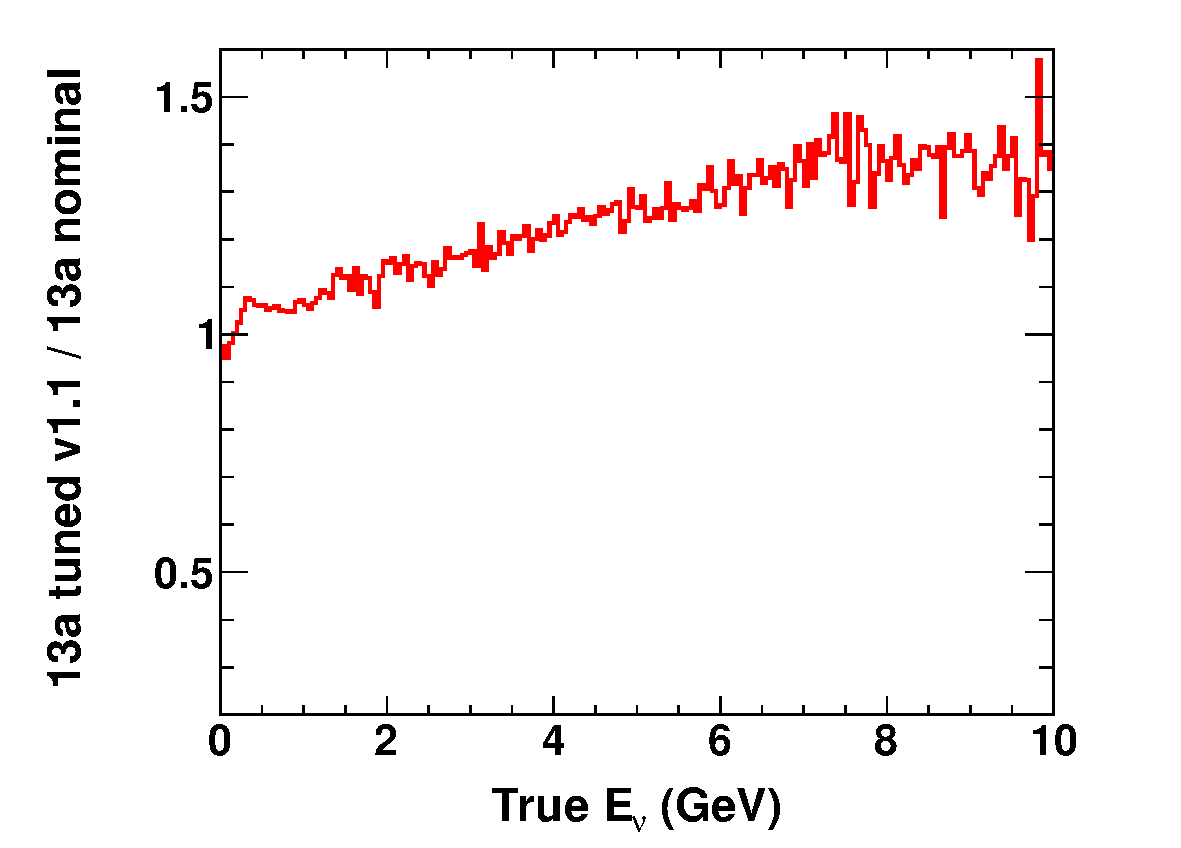
\includegraphics[width=18pc]{./joint_plots/spectrum_predictions/Flux/flux_ratio_13av1p1_to_13anom_numu_numode-eps-converted-to.pdf}
%
\includegraphics[width=18pc]{./images/missing_plot-eps-converted-to.pdf}
\caption {
  $\nu_\mu$ 13a\_v1.1 Run 1-6a flux tuning weights applied to nominal $\nu_\mu$ and oscillated-$\nu_e$ MC templates \cite{FluxTuning13a} (neutrino mode).
  }
\label{fig:na61_weights:numu_numode}
\end{minipage}
\hspace{0.06\linewidth}
\begin{minipage}[t]{0.48\linewidth}
\center
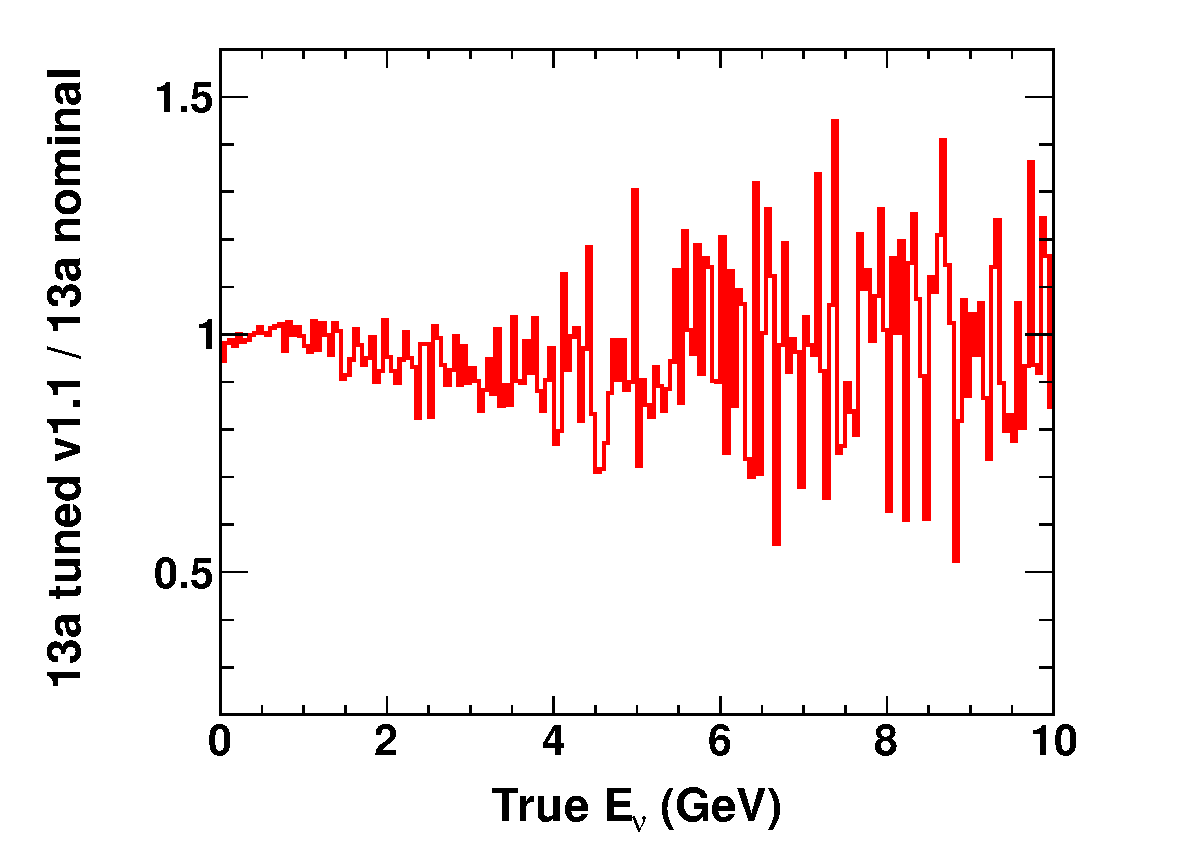
\includegraphics[width=18pc]{./joint_plots/spectrum_predictions/Flux/flux_ratio_13av1p1_to_13anom_numubar_numode-eps-converted-to.pdf}
%
\includegraphics[width=18pc]{./images/missing_plot-eps-converted-to.pdf}
\caption {
  $\bar{\nu}_\mu$ 13a\_v1.1 Run 1-6a flux tuning weights applied to nominal $\bar{\nu}_\mu$ and oscillated-$\bar{\nu}_e$ MC templates \cite{FluxTuning13a} (neutrino mode).
}
\label{fig:na61_weights:numubar_numode}
\end{minipage}
\vfill
\begin{minipage}[t]{0.48\linewidth}
\center
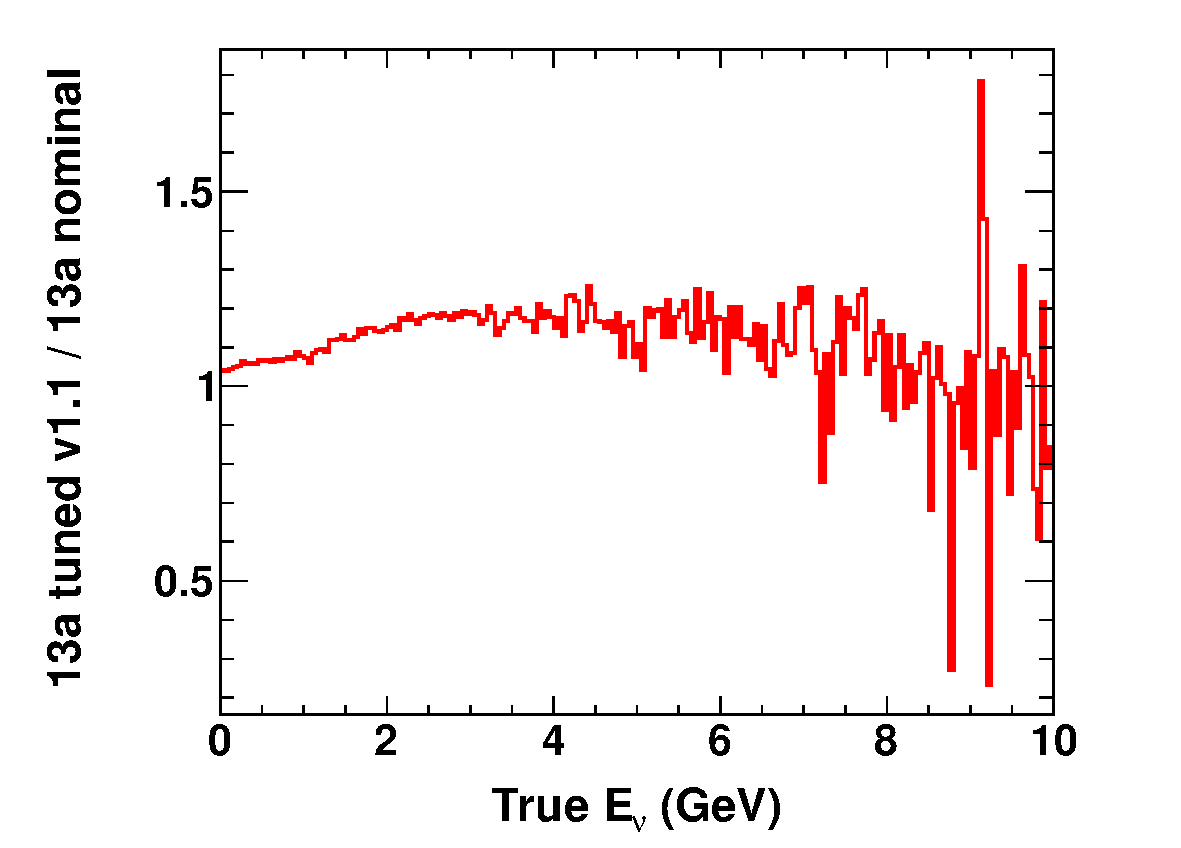
\includegraphics[width=18pc]{./joint_plots/spectrum_predictions/Flux/flux_ratio_13av1p1_to_13anom_nue_numode-eps-converted-to.pdf}
%
\includegraphics[width=18pc]{./images/missing_plot-eps-converted-to.pdf}
\caption {
  $\nu_e$ 13a\_v1.1\ Run 1-6a flux tuning weights applied to nominal $\nu_e$ MC templates \cite{FluxTuning13a} (neutrino mode).
}
\label{fig:na61_weights:nue_numode}
\end{minipage}
\hspace{0.06\linewidth}
\begin{minipage}[t]{0.48\linewidth}
\center
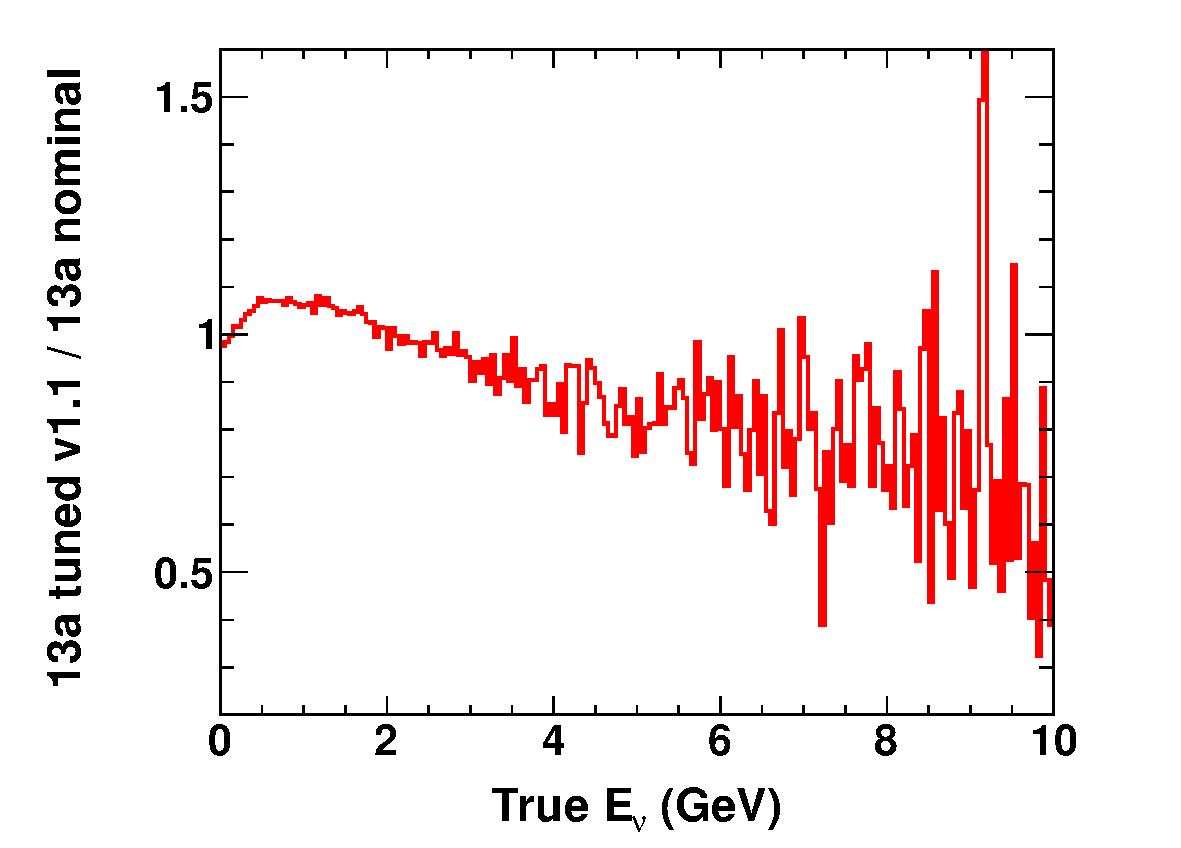
\includegraphics[width=18pc]{./joint_plots/spectrum_predictions/Flux/flux_ratio_13av1p1_to_13anom_nuebar_numode-eps-converted-to.pdf}
%
\includegraphics[width=18pc]{./images/missing_plot-eps-converted-to.pdf}
\caption {
  $\bar{\nu}_e$ 13a\_v1.1 Run 1-6a flux tuning weights applied to nominal $\bar{\nu}_e$ MC templates \cite{FluxTuning13a} (neutrino mode).
}
\label{fig:na61_weights:nuebar_numode}
\end{minipage}
\end{figure*}

%....................................................................................................................


\begin{figure*}[htb]
\begin{minipage}[t]{0.48\linewidth}
\center
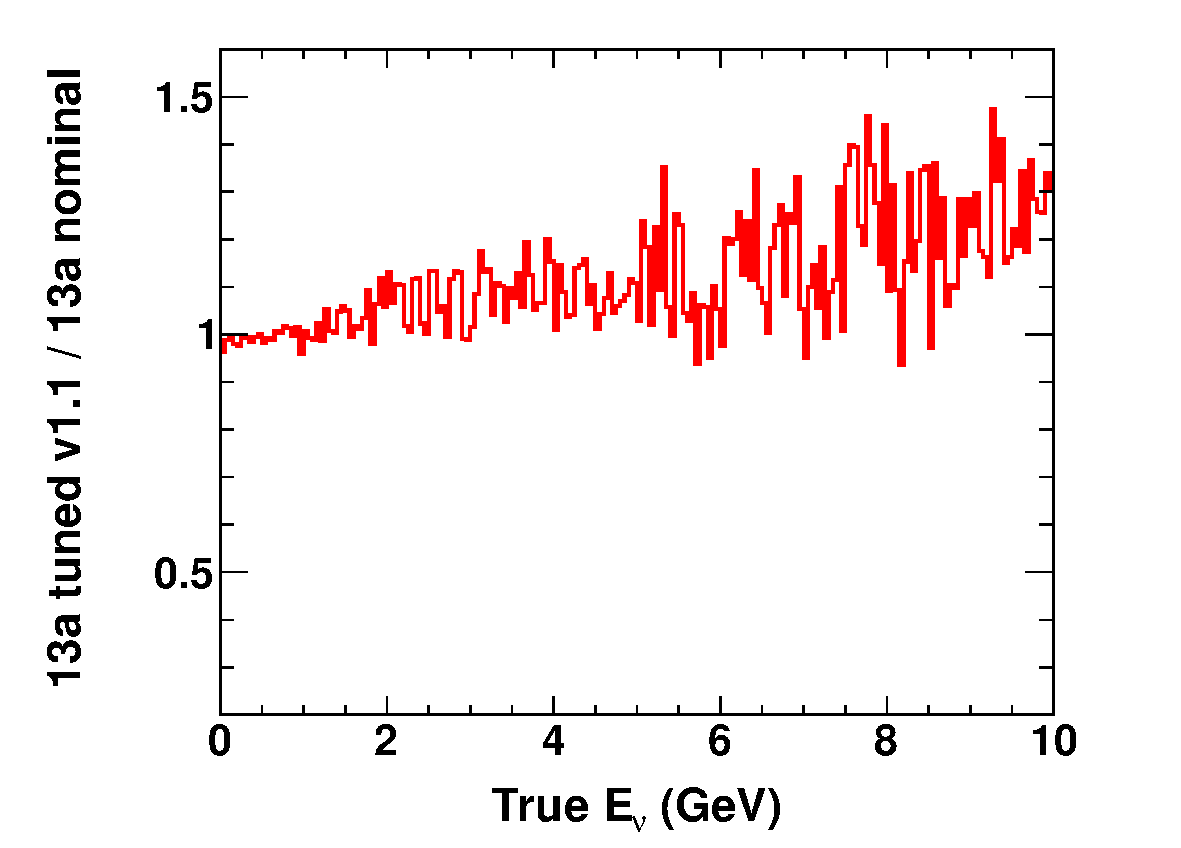
\includegraphics[width=18pc]{./joint_plots/spectrum_predictions/Flux/flux_ratio_13av1p1_to_13anom_numu_nubarmode-eps-converted-to.pdf}
%
\includegraphics[width=18pc]{./images/missing_plot-eps-converted-to.pdf}
\caption {
  $\nu_\mu$ 13a\_v1.1 Run 5c-6b flux tuning weights applied to nominal $\nu_\mu$ and oscillated-$\nu_e$ MC templates \cite{FluxTuning13a} (antineutrino mode).
  }
\label{fig:na61_weights:numu_nubarmode}
\end{minipage}
\hspace{0.06\linewidth}
\begin{minipage}[t]{0.48\linewidth}
\center
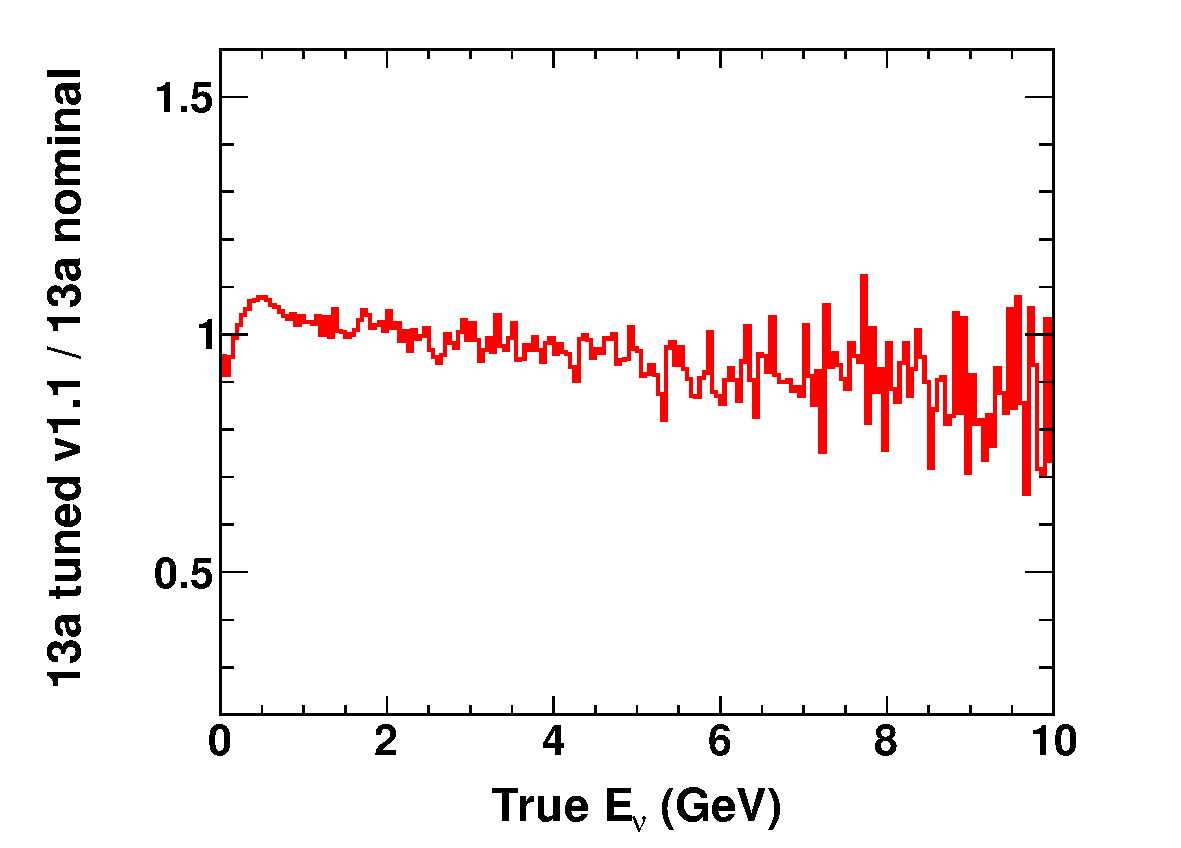
\includegraphics[width=18pc]{./joint_plots/spectrum_predictions/Flux/flux_ratio_13av1p1_to_13anom_numubar_nubarmode-eps-converted-to.pdf}
%
\includegraphics[width=18pc]{./images/missing_plot-eps-converted-to.pdf}
\caption {
  $\bar{\nu}_\mu$ 13a\_v1.1 Run 5c-6b flux tuning weights applied to nominal $\bar{\nu}_\mu$ and oscillated-$\bar{\nu}_e$ MC templates \cite{FluxTuning13a} (antineutrino mode).
}
\label{fig:na61_weights:numubar_nubarmode}
\end{minipage}
\vfill
\begin{minipage}[t]{0.48\linewidth}
\center
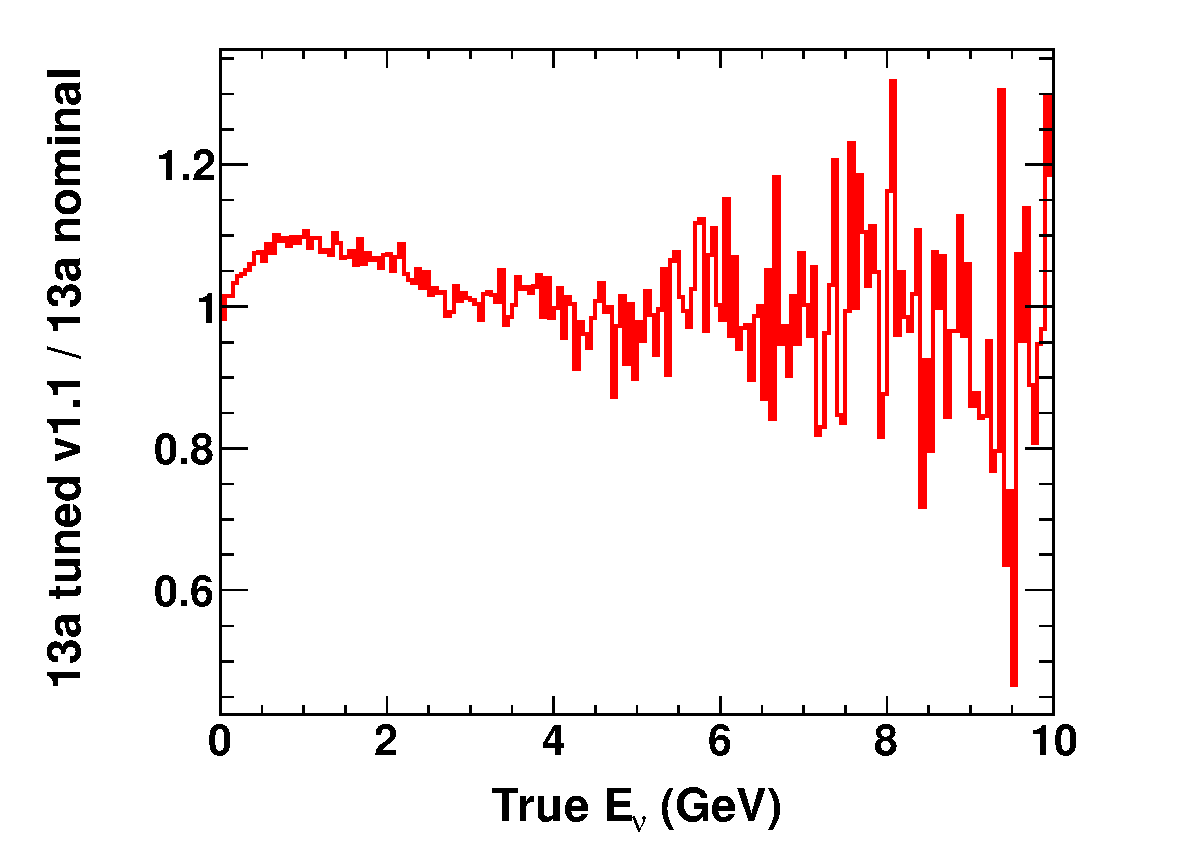
\includegraphics[width=18pc]{./joint_plots/spectrum_predictions/Flux/flux_ratio_13av1p1_to_13anom_nue_nubarmode-eps-converted-to.pdf}
%
\includegraphics[width=18pc]{./images/missing_plot-eps-converted-to.pdf}
\caption {
  $\nu_e$ 13a\_v1.1\ Run 5c-6b flux tuning weights applied to nominal $\nu_e$ MC templates \cite{FluxTuning13a} (antineutrino mode).
}
\label{fig:na61_weights:nue_nubarmode}
\end{minipage}
\hspace{0.06\linewidth}
\begin{minipage}[t]{0.48\linewidth}
\center
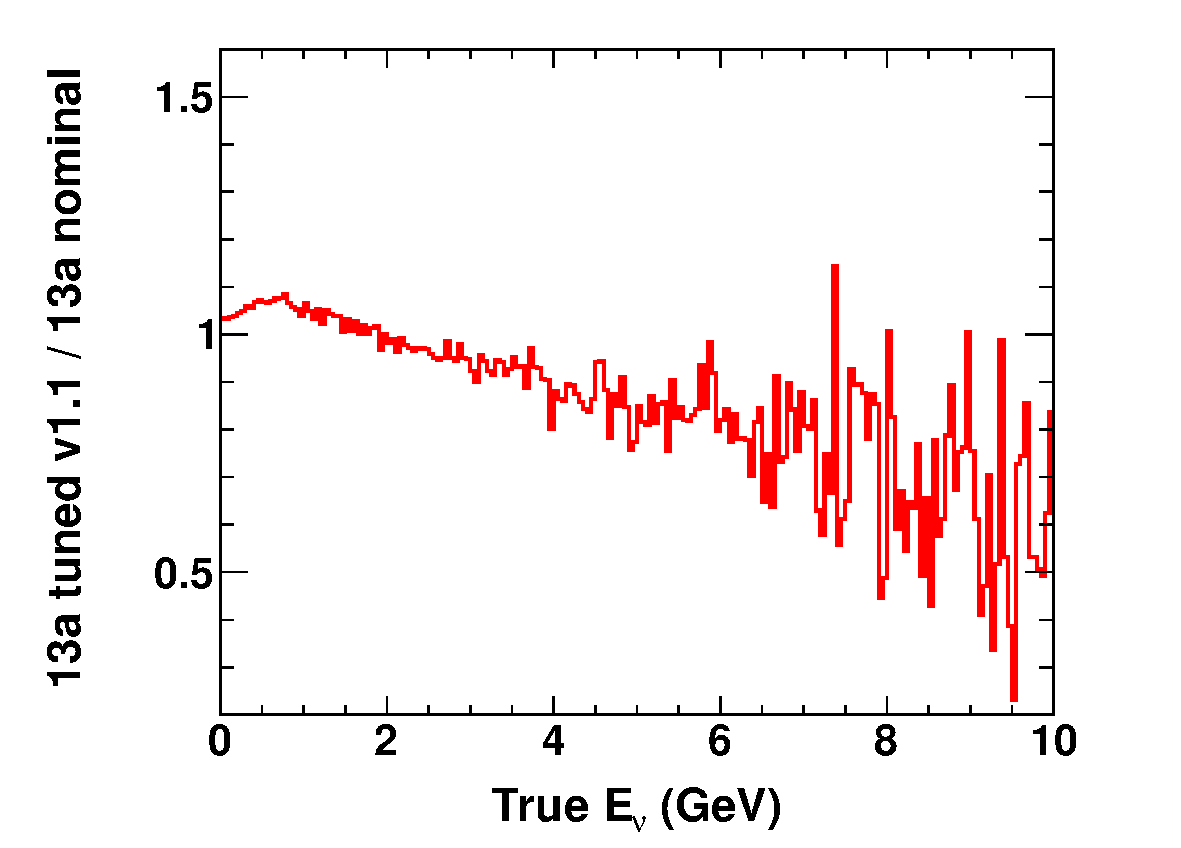
\includegraphics[width=18pc]{./joint_plots/spectrum_predictions/Flux/flux_ratio_13av1p1_to_13anom_nuebar_nubarmode-eps-converted-to.pdf}
%
\includegraphics[width=18pc]{./images/missing_plot-eps-converted-to.pdf}
\caption {
  $\bar{\nu}_e$ 13a\_v1.1 Run 5c-6b flux tuning weights applied to nominal $\bar{\nu}_e$ MC templates \cite{FluxTuning13a} (antineutrino mode).
}
\label{fig:na61_weights:nuebar_nubarmode}
\end{minipage}
\end{figure*}

%....................................................................................................................
%....................................................................................................................

\subsection {Applying flux and cross section (BANFF) tuning based on ND280 data}
\label{sec:banff_weights}

The BANFF group has made a fit of the $\bar{\nu}_\mu$ and  $\nu_\mu$ 
%CC0$\pi$-like, CC1$\pi$-like and CC other 
ND280 samples 
to find the best-fit values of the flux normalisation and cross section parameters \cite{BANFF2015}. This 
analysis uses these best-fit values to reweight the NA61/SHINE-tuned MC templates, and the templates obtained after this second 
reweighting will be denoted the {\em BANFF-tuned} MC templates in this document.
A list of BANFF parameters, their best-fit values and their 1$\sigma$ prefit and postfit errors is given in 
\cref{tab:banff_uncertainties_flux_fhc},~\ref{tab:banff_uncertainties_flux_rhc} and
\ref{tab:banff_uncertainties_xsec}.

The effects of the BANFF tune on the predicted spectra is discussed 
in \cref{sec:nominal_and_tuned_predictions}. 
%(see \cref{fig:1Re_spectrum_w_and_wo_banff_weights} and \cref{tab:nsk_nominal_no_osc} and \cref{tab:nsk_nominal_osc}). 
%....................................................................................................................
%....................................................................................................................


\subsection{Applying neutrino oscillations}
\label{sec:applying_oscillations}

The MC templates are constructed from the unoscillated MC samples and must be weighted with the appropriate oscillation 
probability. Oscillations are applied as a function of true energy to the
%  $\bar{\nu}_{\mu}$ CCQE,
%  $\bar{\nu}_{\mu}$ CC1$\pi$,
%  $\bar{\nu}_{\mu}$ CC coherent,
%  $\bar{\nu}_{\mu}$ CC other,
%  $\nu_{\mu}$ CCQE,
%  $\nu_{\mu}$ CC1$\pi$,
%  $\nu_{\mu}$ CC coherent,
%  $\nu_{\mu}$ CC other,
%  $\bar{\nu}_{e}$ CCQE,
%  $\bar{\nu}_{e}$ CC1$\pi$,
%  $\bar{\nu}_{e}$ CC coherent,
%  $\bar{\nu}_{e}$ CC other
%  $\nu_{e}$ CCQE,
%  $\nu_{e}$ CC1$\pi$,
%  $\nu_{e}$ CC coherent,
%  $\nu_{e}$ CC other,
%  oscillated $\bar{\nu}_{\mu} \rightarrow \bar{\nu}_{e}$ CCQE,
%  oscillated $\bar{\nu}_{\mu} \rightarrow \bar{\nu}_{e}$ CC1$\pi$,
%  oscillated $\bar{\nu}_{\mu} \rightarrow \bar{\nu}_{e}$ CC coherent,
%  oscillated $\bar{\nu}_{\mu} \rightarrow \bar{\nu}_{e}$ CC other,
%  oscillated $\nu_{\mu} \rightarrow \nu_{e}$ CCQE,
%  oscillated $\nu_{\mu} \rightarrow \nu_{e}$ CC1$\pi$,
%  oscillated $\nu_{\mu} \rightarrow \nu_{e}$ CC coherent,
%  oscillated $\nu_{\mu} \rightarrow \nu_{e}$ CC other,
%  oscillated $\nu_{e} \rightarrow \nu_{\mu}$ CCQE,
%  oscillated $\nu_{e} \rightarrow \nu_{\mu}$ CC1$\pi$,
%  oscillated $\nu_{e} \rightarrow \nu_{\mu}$ CC coherent and
%  oscillated $\nu_{e} \rightarrow \nu_{\mu}$ CC other
  MC templates for all CC interactions.

The MC templates calculated from the
$\pbar{\nu}_{\mu}$ MC sample are weighted 
with P($\pbar{\nu}_{\mu} \rightarrow \pbar{\nu}_{\mu}$), with this survival probability being calculated using the 
oscillation parameters, namely $\sin^{2} \theta_{23}$, $\sin^{2} \theta_{12}$, $\sin^{2} \theta_{13}$, 
$|\Delta m^{2}_{32}|$ (normal hierarchy) or $|\Delta m^{2}_{31}|$ (inverted hierarchy), 
$\Delta m^{2}_{21}$ and $\delta_{CP}$. The $\pbar{\nu}_{e}$ templates are weighted with P($\pbar{\nu}_{e} \rightarrow \pbar{\nu}_{e}$), 
while the oscillated $\pbar{\nu}_{\mu} \rightarrow \pbar{\nu}_{e}$ templates are weighted with P($\pbar{\nu}_{\mu} \rightarrow \pbar{\nu}_{e}$) 
(the sample was generated assuming 100\% of $\pbar{\nu}_{\mu}$ transform to $\pbar{\nu}_{e}$). 
%The $\nu_{\mu}$ templates are weighted with P($\nu_{\mu}\rightarrow\nu_{\mu}$). 
%The $\nu_{e}$ templates are weighted with P($\nu_{e}\rightarrow\nu_{e}$) and the 
%oscillated $\nu_{\mu} \rightarrow \nu_{e}$ templates with P($\nu_{\mu}\rightarrow\nu_{e}$).
All these oscillation probabilities are computed in a 3-flavour framework including matter effects in constant-density matter
(assuming an Earth crust density of 2.6 g/cm$^{3}$).
Custom oscillation probability calculation code was developed within the {\em VALOR} analysis framework.
Details and estimates of the numerical accuracy of this code are first presented in \cite{OurRun12DisappAnalysis3Flavour},
and is also shown in Appendix A of \cite{OurRun123DisappAnalysis3Flavour}.
Comparisons between the {\em VALOR} oscillation probability calculation code and Prob3++ \cite{Prob3}, 
which is typically used by the alternative T2K oscillation analyses, are shown in Appendix B of \cite{OurRun123DisappAnalysis3Flavour}.

In the standard 3-flavour oscillation framework,
oscillations of $\pbar{\nu}_{e}$ and $\pbar{\nu}_{\mu}$ can yield $\pbar{\nu}_{\tau}$.
In this analysis, we neglect contributions from $\nu_{\tau}$-CC and $\bar{\nu}_{\tau}$-CC as their
energy threshold is around 3.5 GeV and their effect is negligible\footnote{
A back-of-the-envelope calculation can be found in the replies to
comments and revision history document of
\cite{OurRun123DisappAnalysis3Flavour} that gives $\ll 1\%$ $\nu_\tau$
contamination in the 1-ring $\mu$-like Super-K sample. A Super-K MC study is required
to determine whether the Super-K efficiency assumptions made there are valid.
  }.
Accordingly, this analysis uses no $\nu_{\tau}$-CC and $\bar{\nu}_{\tau}$-CC MC templates
(and, in fact, no $\nu_{\tau}$ and $\bar{\nu}_{\tau}$ Super-K MC samples are available).

It should be emphasized here that
the $\nu_{\mu}$ NC MC templates for a mode $m$ contain the
NC MC templates for the mixture of $\nu_{e}$+$\nu_{\mu}$+$\nu_{\tau}$ resulting from
3-flavour $\nu_{\mu}$ oscillations for that mode $m$. The same applies to the $\bar{\nu}_{\mu}$, $\nu_{e}$ and $\bar{\nu}_{e}$ 
NC MC templates. These NC MC templates are unchanged under standard 3-flavour oscillations.% (see also \cref{sec:}).

Also it should be noted that there are no explicit NC MC templates made from the oscillated $\bar{\nu}_{e}$ and $\nu_{e}$ 
samples. If they were used, the oscillated $\bar{\nu}_{e}$ (i.e.\ $\bar{\nu}_{e}$ coming from oscillations of $\bar{\nu}_{\mu}$) 
would be double counted since they are already included in the $\bar{\nu}_{\mu}$ NC MC templates. The same applies to oscillated 
$\nu_{e}$.

%....................................................................................................................
%....................................................................................................................

\subsection {Predictions of nominal and tuned-MC spectra}
\label{sec:nominal_and_tuned_predictions}

In this section, we present the expected spectra in Super-K for various oscillation scenarios. 
%We also present estimates of the effect of the NA61/SHINE and BANFF tunings and of assumptions 
%made in the 3-flavour neutrino oscillation framework used in this analysis. 
Unless explicitly stated otherwise, the oscillation 
parameters are set to the Asimov data set A shown in \cref{tab:osc_params_joint_asimov} and the normal mass hierarchy is assumed.
All plots are generated for an integrated exposure 
corresponding to Run 1-7c.
%of \TotalPotNu{} POT for neutrino and \TotalPotNuBar{} POT for antineutrino mode.


Predicted single ring Super-K spectra are shown in \cref{fig:joint_ereco_vs_theta_all}. 
By comparing neutrino and antineutrino mode $e$-like plots it is clear that $E_{reco}$ vs $\theta$ distributions are differently populated
by $\nu_{\mu} \rightarrow \nu_e$ and $\bar{\nu}_{\mu} \rightarrow \bar{\nu}_e$ events.
\textbf{More details on the advantage of the 2-dimensional templates are given in appendix~\ref{app:templates_elike}.}

%for oscillations assuming the normal hierarchy and the oscillation parameters shown in \cref{tab:osc_params_joint}.

\begin{figure*}[htb]
\center
\begin{subfigure}[b]{0.49\textwidth}
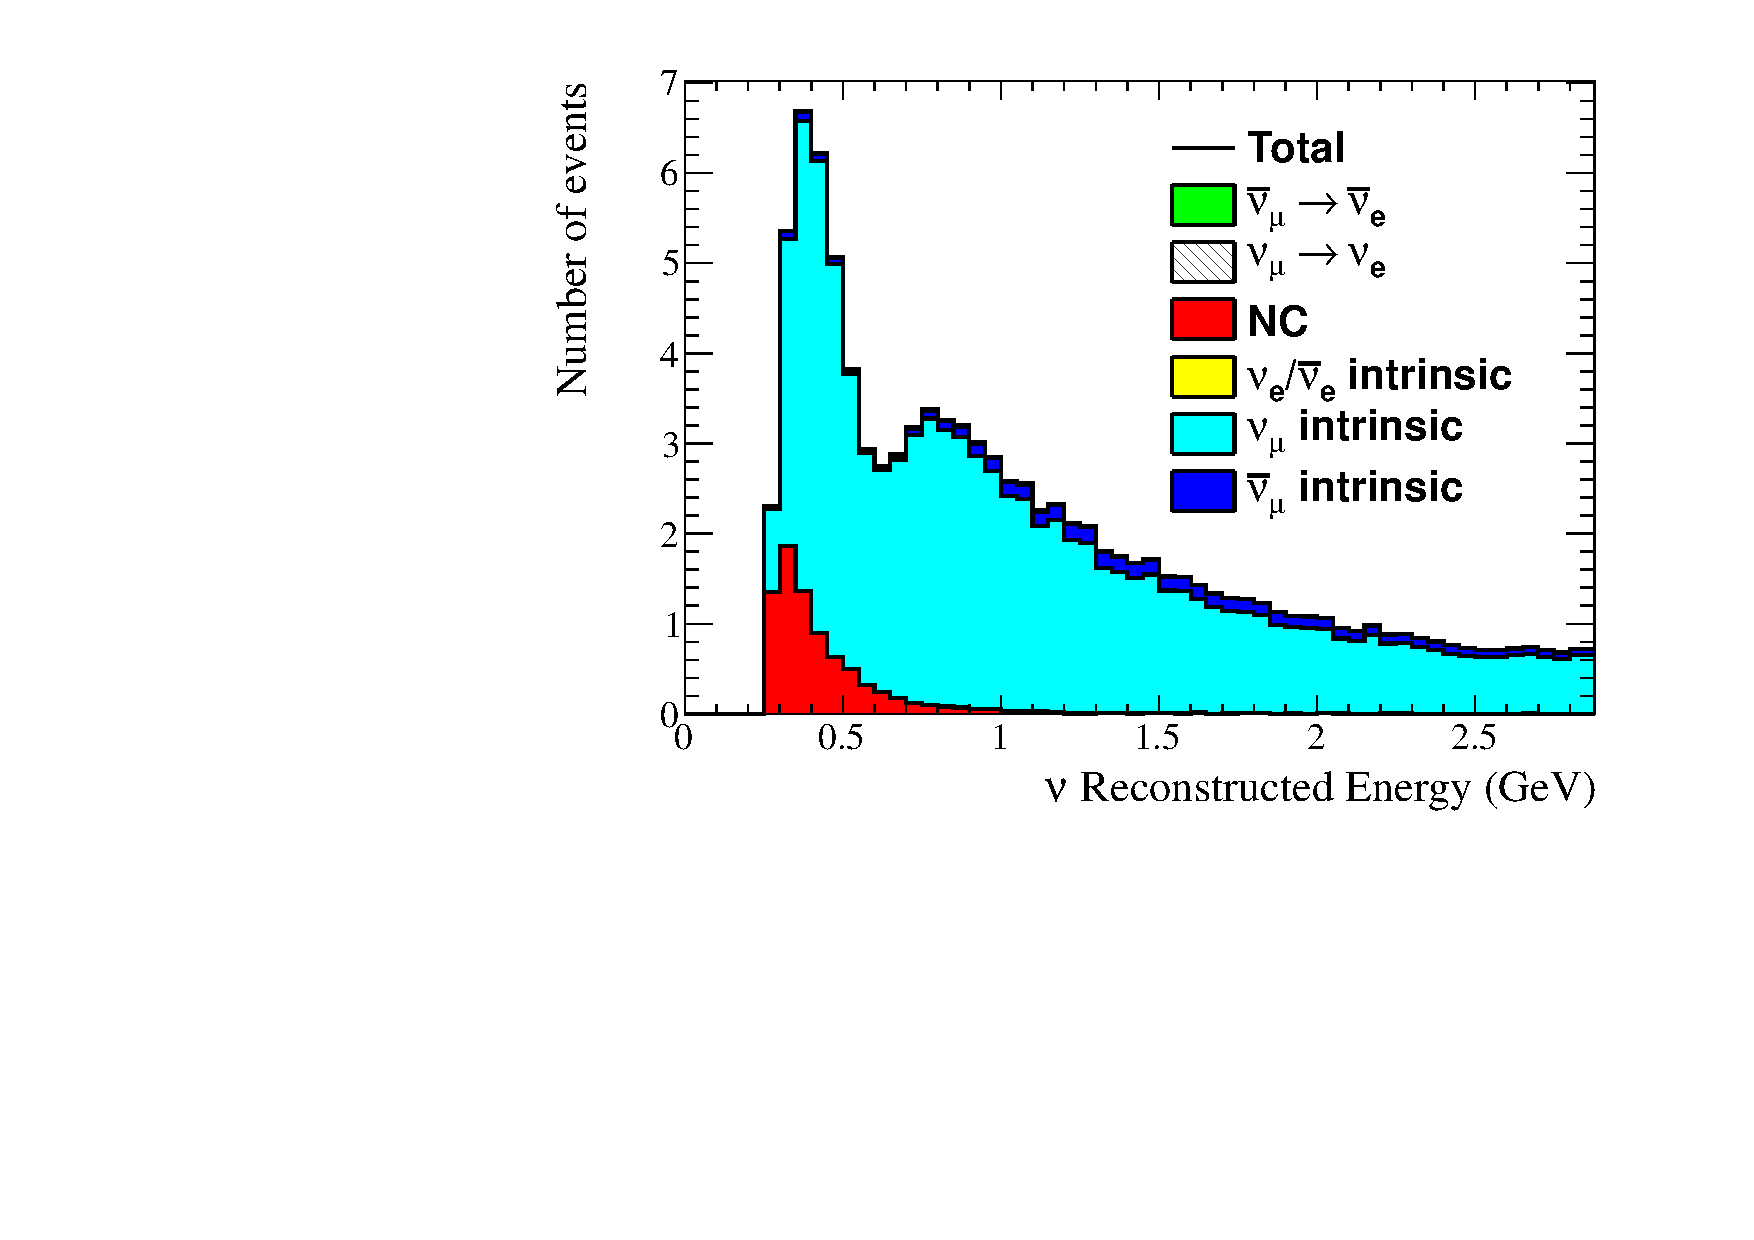
\includegraphics[width=0.9\textwidth]{joint_plots/spectrum_predictions/template_ereco_1rmu_zoom.pdf}
\caption{Muon-like, neutrino mode}
\end{subfigure}
\begin{subfigure}[b]{0.49\textwidth}
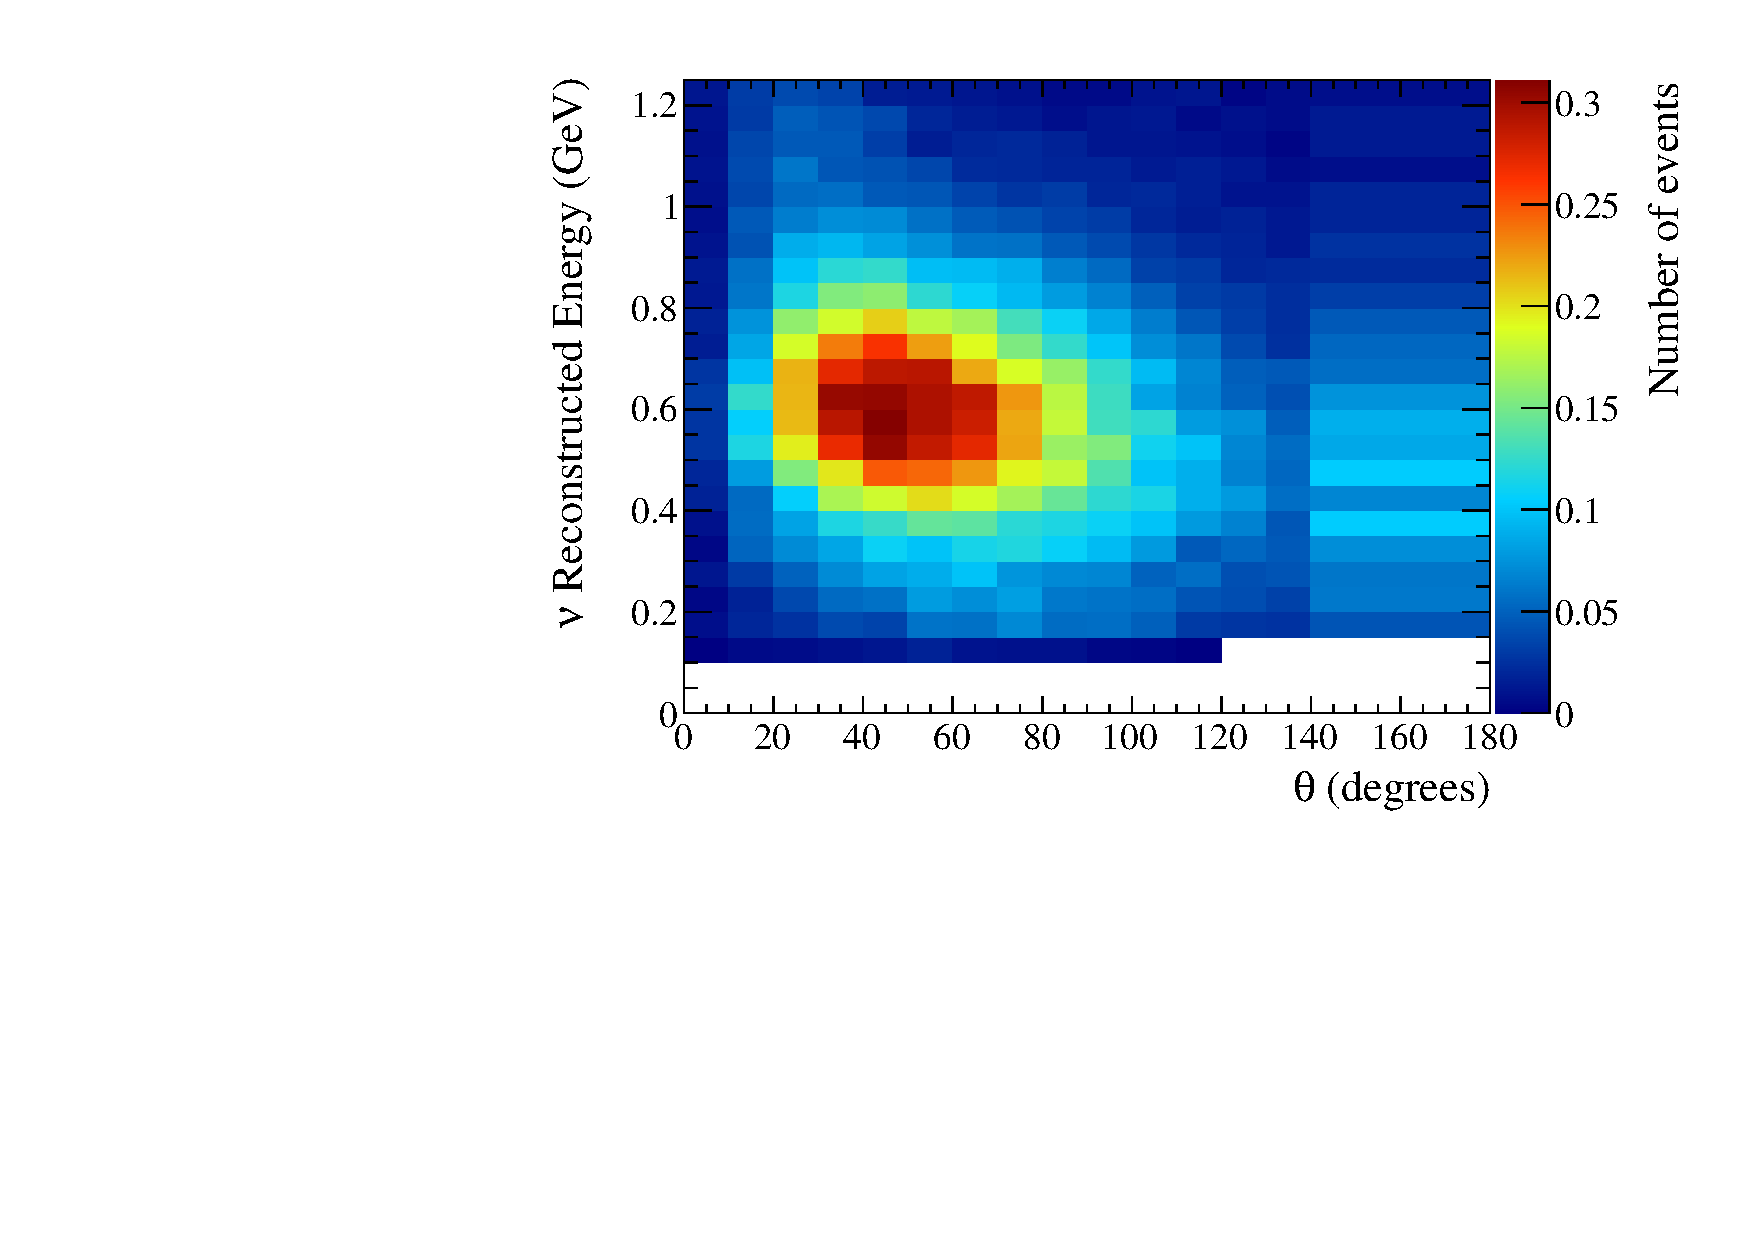
\includegraphics[width=0.9\textwidth]{joint_plots/spectrum_predictions/template_ereco_vs_theta_tot_1re.pdf}
\caption{Electron-like, neutrino mode}
\end{subfigure}
\begin{subfigure}[b]{0.49\textwidth}
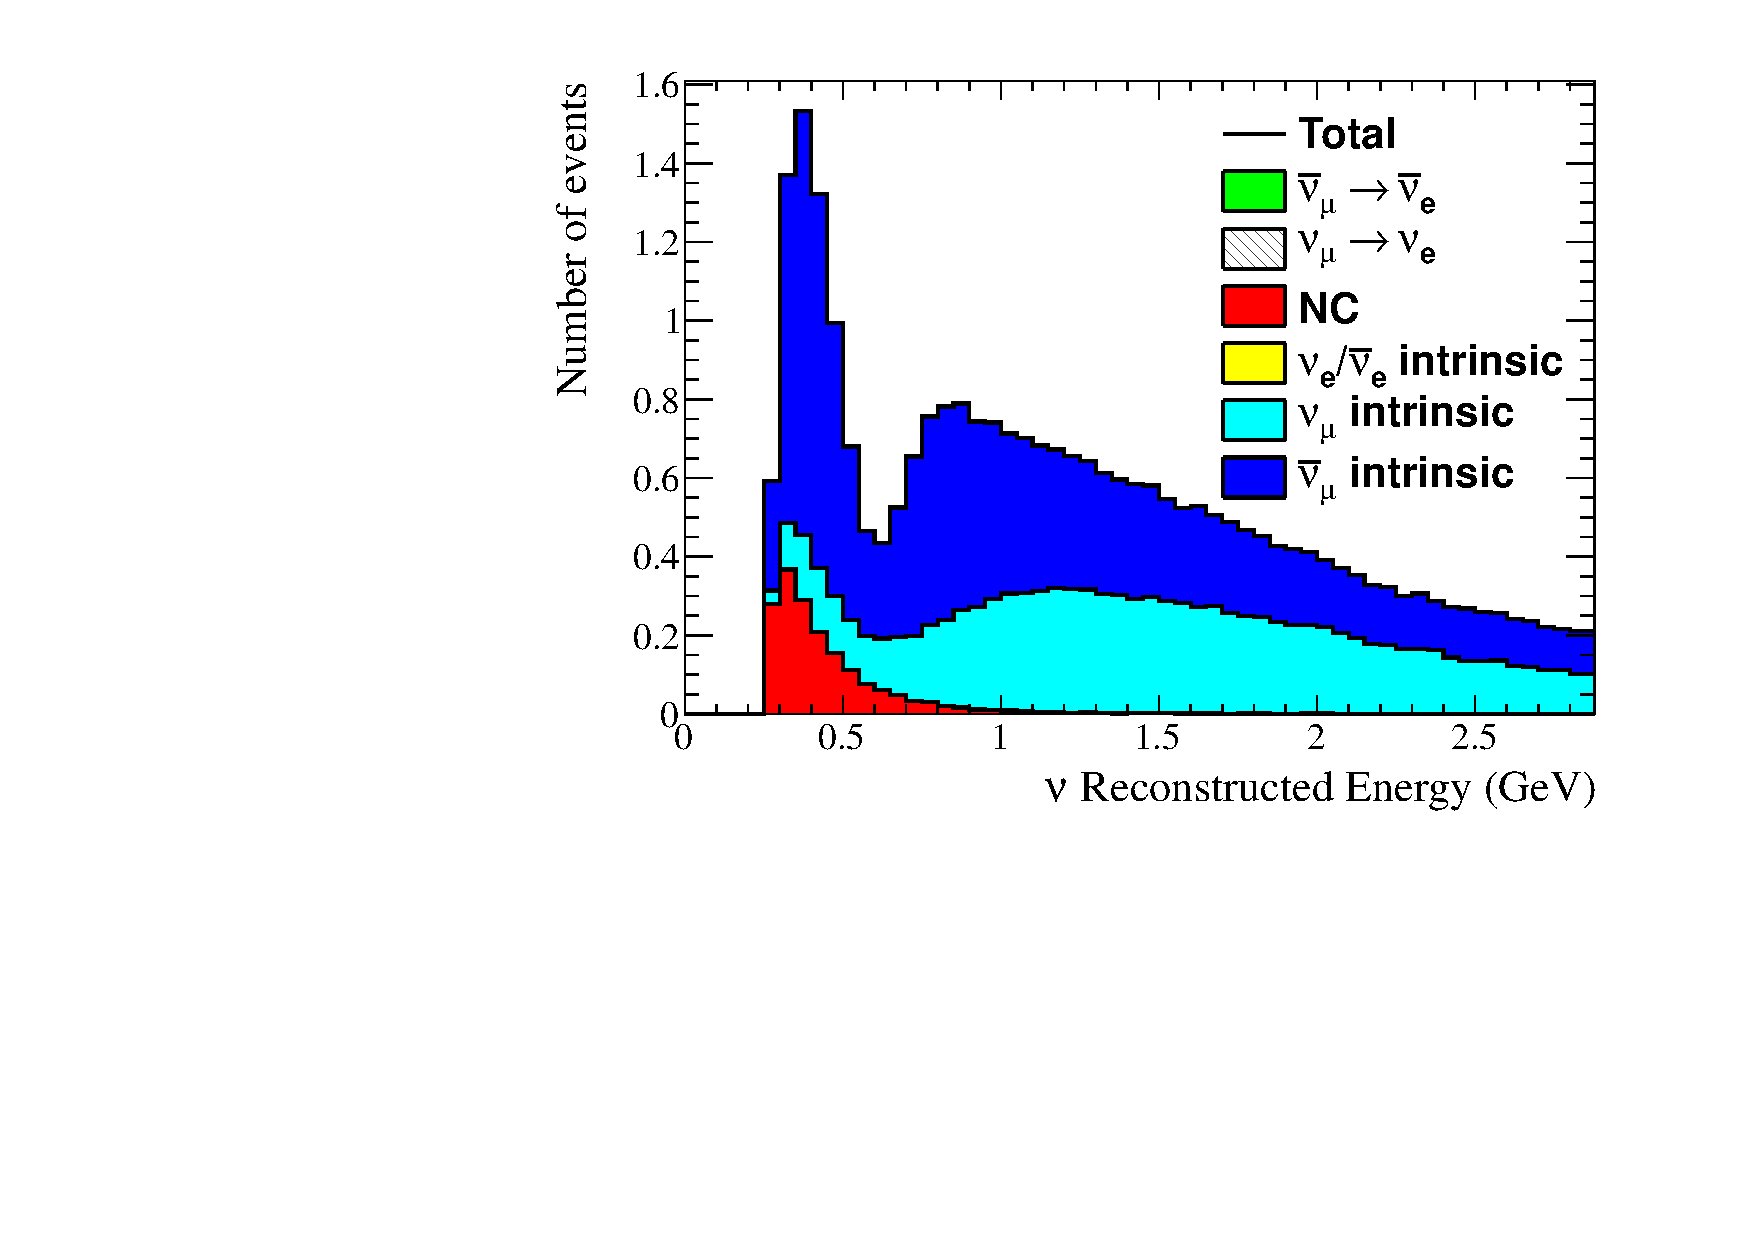
\includegraphics[width=0.9\textwidth]{joint_plots/spectrum_predictions/template_ereco_rhc1rmu_zoom.pdf}
\caption{Muon-like, antineutrino mode}
\end{subfigure}
\begin{subfigure}[b]{0.49\textwidth}
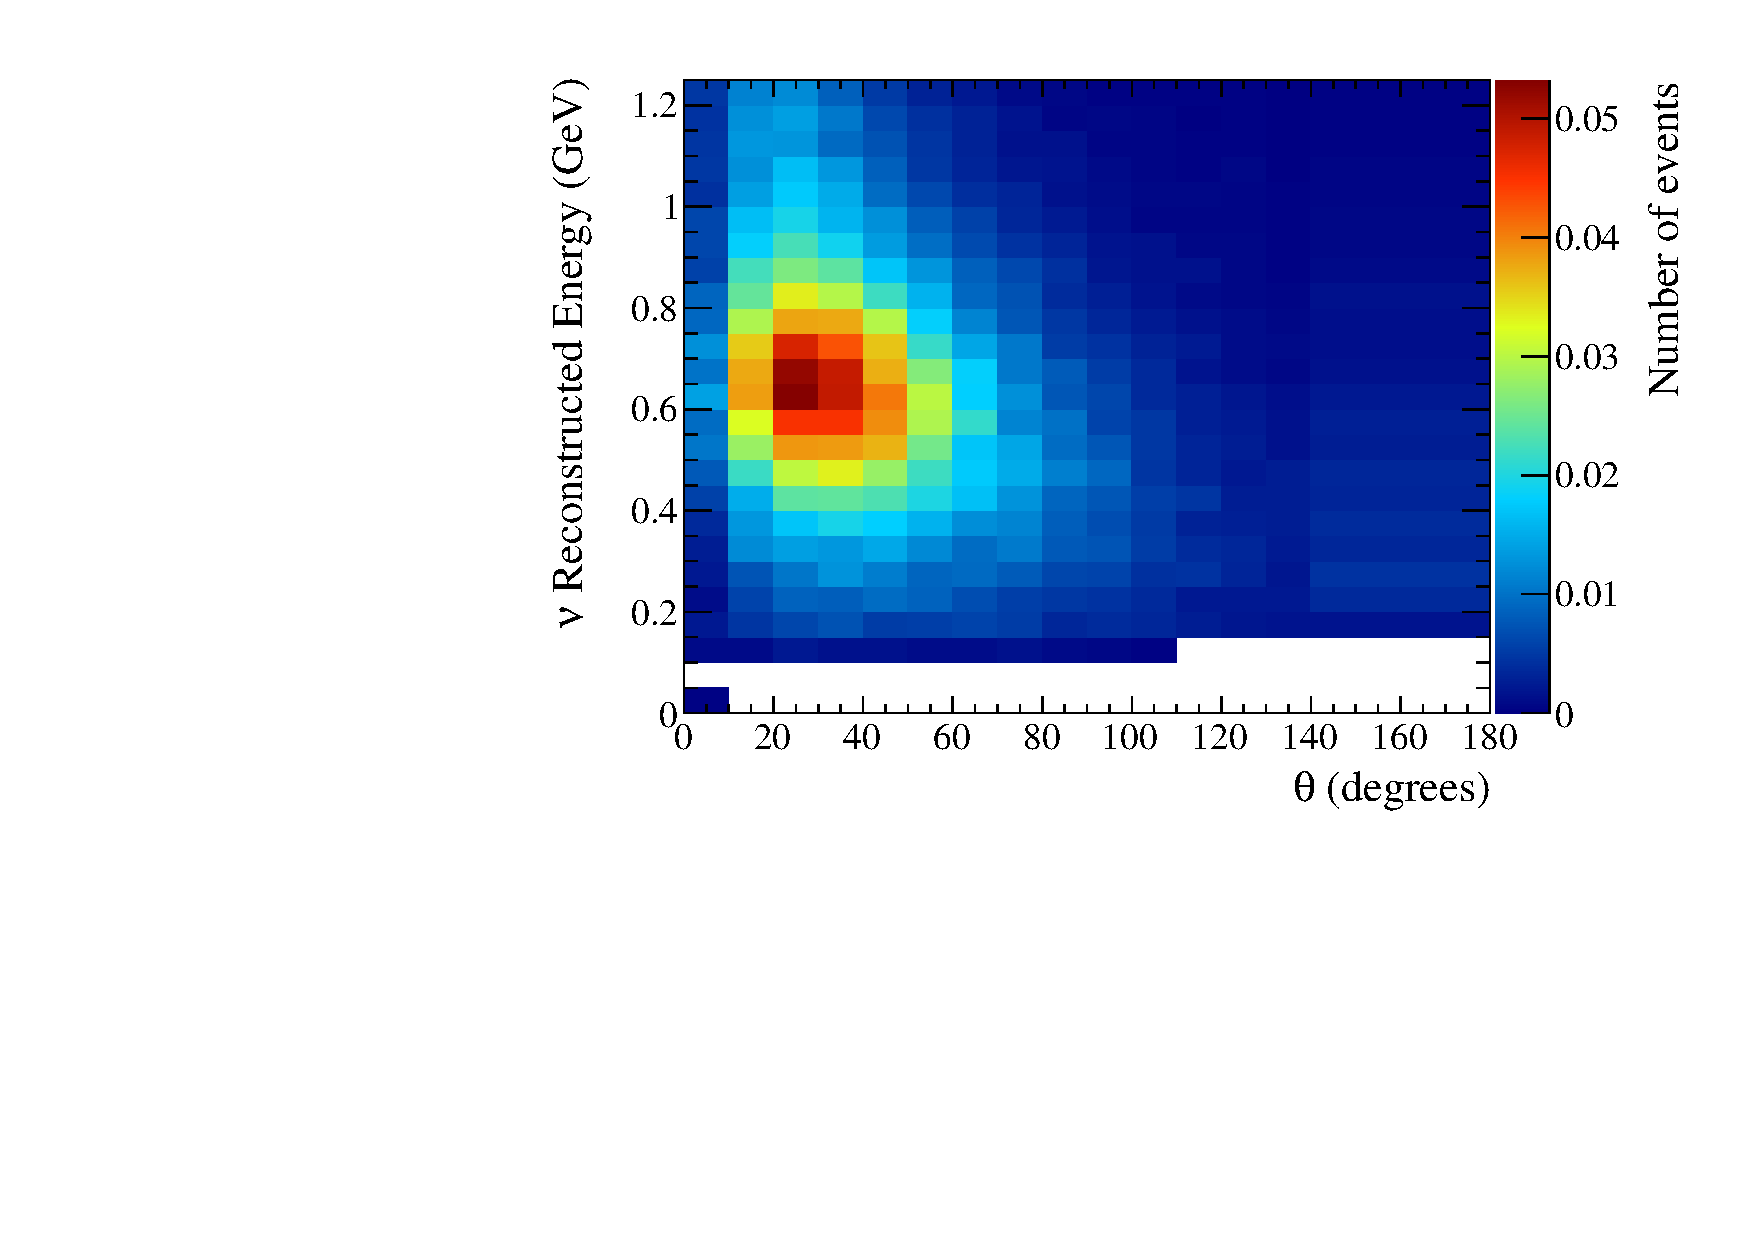
\includegraphics[width=0.9\textwidth]{joint_plots/spectrum_predictions/template_ereco_vs_theta_tot_rhc1re.pdf}
\caption{Electron-like antineutrino mode}
\end{subfigure}
\begin{subfigure}[b]{0.49\textwidth}
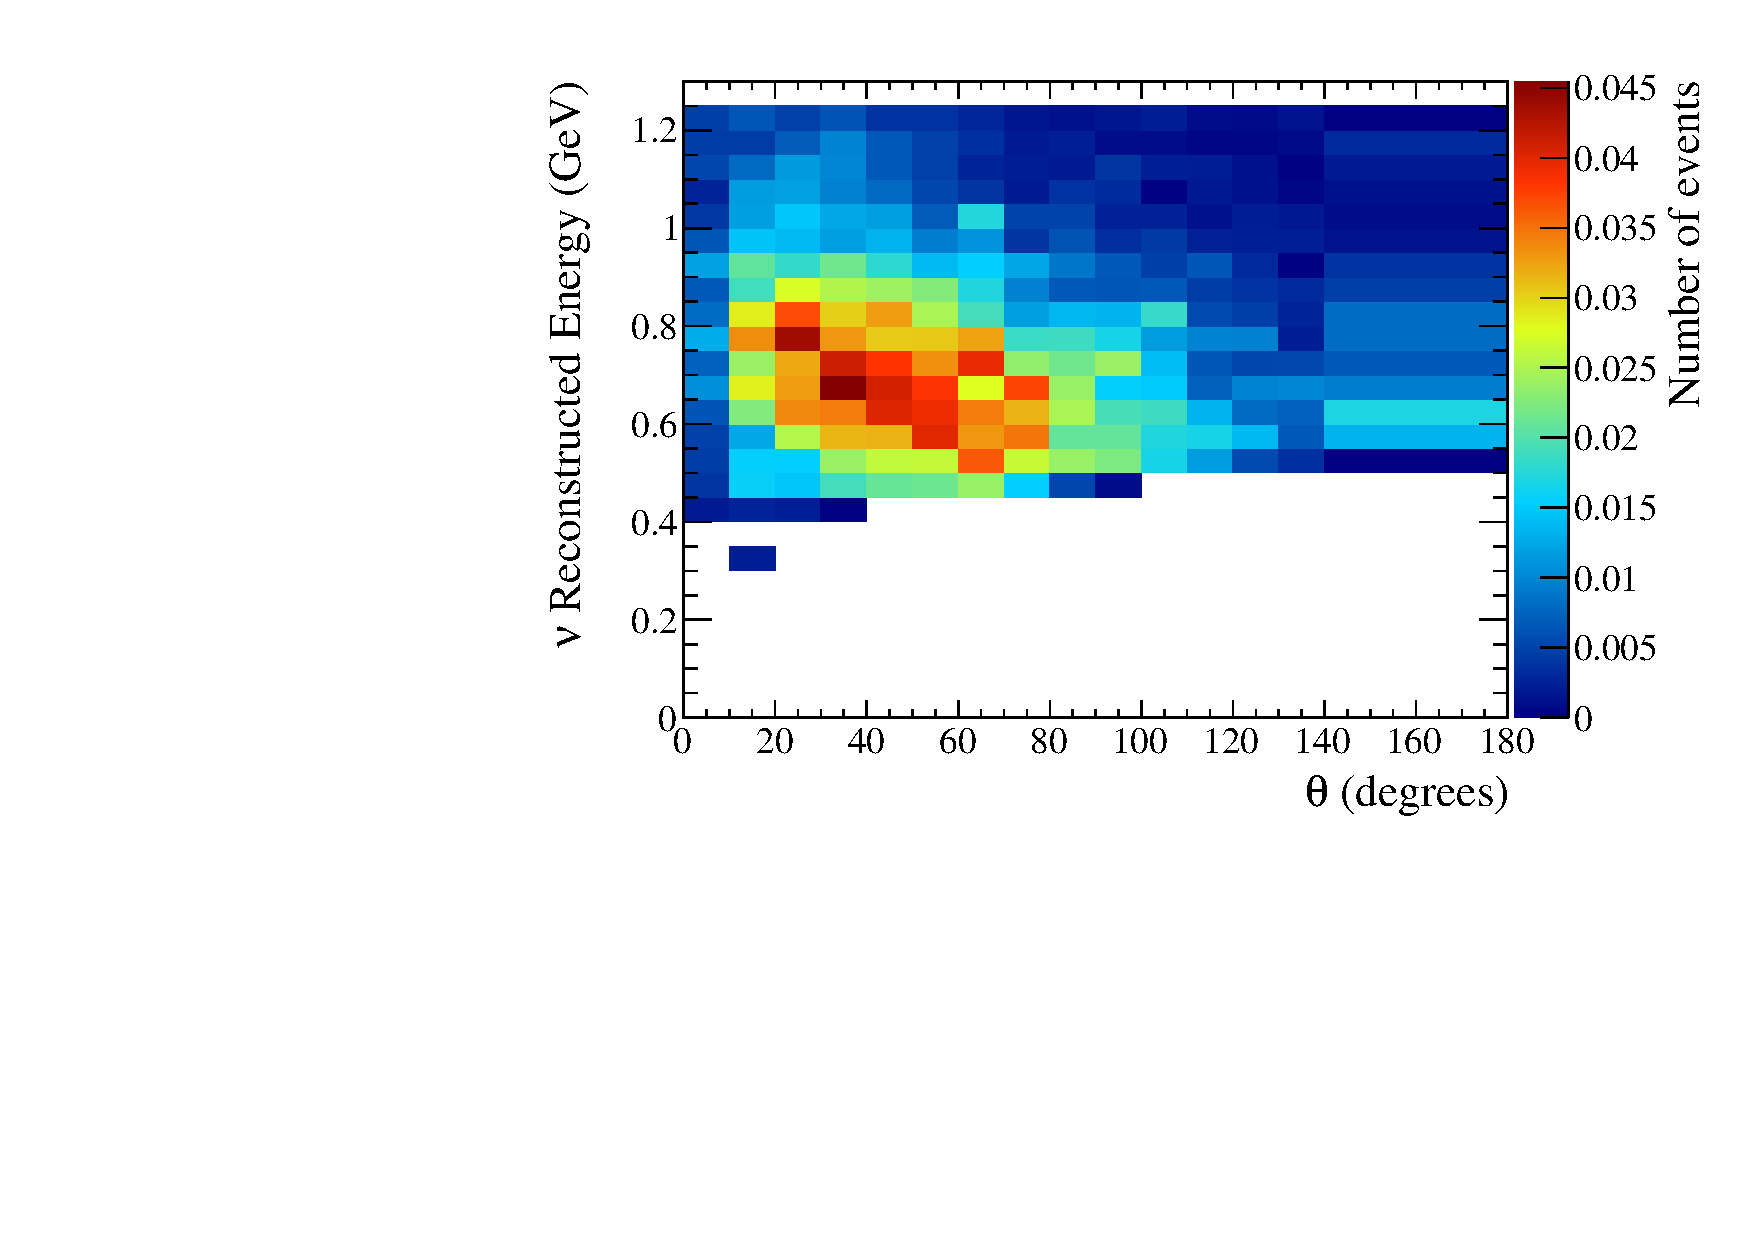
\includegraphics[width=0.9\textwidth]{joint_plots/spectrum_predictions/template_theta_ccpi.pdf}
\caption{\nueCConepi-like, neutrino mode}
\end{subfigure}
\caption {
Predicted spectra, muon-like distributions are function of the reconstructed neutrino energy,
while the electron-like, including \nueCConepi, distributions are function of both the reconstructed neutrino energy and
the reconstructed angle between the outgoing lepton and the neutrino direction.
The distributions correspond to the statistics collected in the full Run 1-7c data set.
%for an exposure 
%of $6.914 \times 10^{20}$ POT in neutrino mode
%and
%of $4.011 \times 10^{20}$ POT in antineutrino mode.
The muon-like distributions are broken down by the following components:
$\bar{\nu}_{\mu} \to \bar{\nu}_e$ (green), 
$\nu_{\mu} \to \nu_e$ (black/white), 
NC (red),
$\nu_e + \bar{\nu}_e$ intrinsic beam (yellow),
$\nu_{\mu}$ intrinsic beam (light blue)
and
$\bar{\nu}_{\mu}$ intrinsic beam (blue).
The spectra are generated with the systematic parameters measured with the ND280 data 
shown in 
\cref{tab:banff_uncertainties_flux_fhc},~\ref{tab:banff_uncertainties_flux_rhc},
\ref{tab:banff_uncertainties_xsec} and the nominal Super-K systematic parameters shown in ~\cref{tab:banff_uncertainties_skdetfsi}
and the oscillation parameters corresponding to the Asimov data set A 
shown in \cref{tab:osc_params_joint_asimov}.
}
\label{fig:joint_ereco_vs_theta_all}
\end{figure*}















%A MC tune derived using NA61/SHINE data is applied to the nominal MC templates, and another tune derived using the ND280 data is 
%applied to the NA61/SHINE-tuned templates as described in \cref{sec:na61_weights} and \cref{sec:banff_weights}.
%%
%The fractional difference in the expected number of single $e$-like ring events when switching from the nominal MC to the
%NA61/SHINE-tuned MC templates is shown in \cref{fig:1Re_spectrum_w_and_wo_na61_weights} 
%both oscillated and not oscillated. 
%%In \cref{fig:1Re_spectrum_w_and_wo_banff_weights} it is shown the fractional difference in the expected number of
%%single-ring $e$-like events when switching from the NA61/SHINE-tuned MC templates to the BANFF-tuned MC templates.
%In \cref{fig:1Re_spectrum_w_and_wo_na61_weights} it is shown the fractional difference in the expected number of single-ring e-like events
%when switching from the nominal MC templates to NA61/SHINE-tuned MC templates.
%%
%The effects of the NA61/SHINE and BANFF tunes on the total expected number of single-ring $e$-like events
%and on the numbers in each of the \NMCTemplate{} component interaction modes are shown in
%\cref{tab:nsk_nominal_no_osc} for no oscillations, and in
%\cref{tab:nsk_nominal_osc} for oscillations assuming the normal hierarchy, and the oscillation parameters shown in \cref{tab:osc_params_fixed_values_reactor}.
%Finally, the effects of the NA61/SHINE and BANFF tunes on the reconstructed energy spectrum of
%single $e$-like ring events are shown in
%\cref{fig:1Re_spectrum_w_and_wo_banff_weights}.
%In each case, spectra are shown for both no oscillations and for oscillations assuming the normal hierarchy, and the oscillation parameters shown in \cref{tab:osc_params_fixed_values_reactor}.
%%Also shown are the ratio of flux-tuned spectrum to nominal spectrum, and
%%BANFF-tuned spectrum to flux-tuned spectrum in \cref{fig:1Re_spectrum_w_and_wo_banff_weights}.
%Also shown are the ratio of BANFF-tuned spectrum to flux-tuned spectrum in \cref{fig:1Re_spectrum_w_and_wo_banff_weights}.

%%% Local Variables:
%%% mode: latex
%%% TeX-master: "jointfit_5sample2016"
%%% End:
